\documentclass[twoside]{book}

% Packages required by doxygen
\usepackage{fixltx2e}
\usepackage{calc}
\usepackage{doxygen}
\usepackage[export]{adjustbox} % also loads graphicx
\usepackage{graphicx}
\usepackage[utf8]{inputenc}
\usepackage{makeidx}
\usepackage{multicol}
\usepackage{multirow}
\PassOptionsToPackage{warn}{textcomp}
\usepackage{textcomp}
\usepackage[nointegrals]{wasysym}
\usepackage[table]{xcolor}

% NLS support packages
% Font selection
\usepackage[T1]{fontenc}

\usepackage[scaled=.90]{helvet}
\usepackage{courier}
\usepackage{amssymb}
\usepackage{sectsty}
\renewcommand{\familydefault}{\sfdefault}
\allsectionsfont{%
  \fontseries{bc}\selectfont%
  \color{darkgray}%
}
\renewcommand{\DoxyLabelFont}{%
  \fontseries{bc}\selectfont%
  \color{darkgray}%
}
\newcommand{\+}{\discretionary{\mbox{\scriptsize$\hookleftarrow$}}{}{}}

% Page & text layout
\usepackage{geometry}
\geometry{%
  a4paper,%
  top=3cm,%
  bottom=2cm,%
  left=3cm,%
  right=2cm%
}
\tolerance=750
\hfuzz=15pt
\hbadness=750
\setlength{\emergencystretch}{15pt}
\setlength{\parindent}{0cm}
\setlength{\parskip}{3ex plus 2ex minus 2ex}
\makeatletter
\renewcommand{\paragraph}{%
  \@startsection{paragraph}{4}{0ex}{-1.0ex}{1.0ex}{%
    \normalfont\normalsize\bfseries\SS@parafont%
  }%
}
\renewcommand{\subparagraph}{%
  \@startsection{subparagraph}{5}{0ex}{-1.0ex}{1.0ex}{%
    \normalfont\normalsize\bfseries\SS@subparafont%
  }%
}
\makeatother



% Hyperlinks (required, but should be loaded last)
\usepackage{ifpdf}
\ifpdf
  \usepackage[pdftex,pagebackref=true]{hyperref}
\else
  \usepackage[ps2pdf,pagebackref=true]{hyperref}
\fi
\hypersetup{%
  colorlinks=true,%
  linkcolor=blue,%
  citecolor=blue,%
  unicode%
}

% Custom commands
\newcommand{\clearemptydoublepage}{%
  \newpage{\pagestyle{empty}\cleardoublepage}%
}
\usepackage{caption}
\captionsetup{labelsep=space,font={bf},singlelinecheck=off,position=top}

%===== C O N T E N T S =====

\begin{document}

% Titlepage & ToC
\hypersetup{pageanchor=false,
             bookmarksnumbered=true,
             pdfencoding=unicode
            }
\pagenumbering{alph}
\begin{titlepage}
\vspace*{7cm}
\begin{center}%
{\Large Analytics -\/ Estrutura de Dados \\[1ex]\large 1.\+0.\+0-\/alpha }\\
\vspace*{1cm}
{\large Augusto Zanella Bardini}\\
{\large Rafael Baldasso Audibert}\\
\end{center}
\end{titlepage}
\pagenumbering{roman}
\clearemptydoublepage
\pagenumbering{arabic}
\hypersetup{pageanchor=true}

%--- Begin generated contents ---
\chapter{Analytics -\/ Estruturas de Dados}
\label{md__r_e_a_d_m_e}

\Hypertarget{md__r_e_a_d_m_e}
\subsection*{Descrição}

O presente trabalho tem como objetivo a implementação de um “Analytics” de um motor de busca, onde são recebidas consultas realizadas e gera-se então um relatório a respeito dos dados inseridos durante a consulta.

Esse relatório é gerado com base em operações que podem ser realizadas com as consultas. Essas operações são: (a) consultas mais realizadas por localidade; (b) consultas mais realizadas em todo o arquivo; (c) termos mais consultados por localidade; (d) termos mais consultados em todo o arquivo; (e) tamanho médio das consultas por localidade; e (f) tamanho médio das consultas no arquivo.

Ao final do programa, também é dado como feedback o tempo gasto, tanto da leitura/manipulação de entrada dos dados, como do tempo gasto para realizar as operações nesses dados.

\subsection*{Implementação}

O programa utiliza como estrutura de dados principal uma ABP cujos nós são as diferentes consultas realizadas. A ABP é ordenada pela quantidade de termos de cada consulta (nó).

Em cada nó da árvore, a consulta fica organizada por termos dentro de uma Lista Simplesmente Encadeada. Nesse mesmo nó, há também uma Lista Duplamente Encadeada que armazena as cidades nas quais foi realizada aquela consulta, guardando na mesma lista quantas vezes aquela cidade realizou a consulta. Temos também um valor que guarda a quantidade de acessos geral para aquela consulta, independentemente de cidade.

Para facilitar algumas operações, também foi criada uma Lista Duplamente Encadeada geral, que armazena TODOS os termos que foram consultados no arquivo, assim como a quantidade de vezes que ele foi consultado.

Na hora de realizar as operações, já temos acesso a toda essa informação gerada na inserção dos dados, porém não temos todas saídas de operação definidas separadamente. Para cada uma das operações, varremos a estrutura de árvores de listas buscando os dados necessários. Apenas uma operação utiliza de uma estratégia diferente: Consultas mais realizadas em todo o arquivo. Assim que é entrada na fase de realizar as operações, imediatamente é chamada a função que percorre todas as consultas, as transforma em strings, e as deixa ordenadas em em função de maior ocorrência. O motivo de ser realizado isso, é que em um arquivo com 4800 consultas diferentes, todo esse processo leva cerca de 1,5 segundos, logo, é necessário poupar tempo, mantendo as consultas salva em um “cache”, tornando a chegada no resultado mais simples.

Para as outras operações, foram criadas funções que procuram os valores corretos a cada diferente operação, sem a utilização de algo parecido com um “cache”.

\subsection*{Idealização inversa}

A ideia de colocar na ABP as consultas, e não as cidades, como seria intuitivo fazer, dada a definição do trabalho, surgiu pensando que teríamos muitas consultas semelhantes de várias cidades diferentes, o que tornaria o código possivelmente muito mais rápido em comparação com o formato de árvore de cidades. Porém, ao serem definidas como entrada consultas, implicando muitas consultas diferentes e poucas cidades diferentes em cada consulta, nosso código tende a levar mais tempo do que programas otimizados para menos cidades/mais consultas.

\subsection*{Conclusão}

Mesmo não tendo sido implementado uma árvore balanceada, ou que facilitasse o acesso a consultas, como uma árvore AVL, ou Splay, respectivamente, pode-se perceber quão rápido a árvore deixa o programa em comparação a uma lista simplesmente encadeada, uma vez que não é necessário percorrer todos os nós para encontrar o nó necessário para determinada ação. Certamente, um programa feito baseado inteiramente em listas demoraria muito mais tempo para realizar operações com uma grande quantidade de dados, como foi utilizado durante a execução desse trabalho.

A nível de complexidade, o trabalho mostrou que estruturas de armazenamento de vários tipos de dados se tornam inevitavelmente complexas, principalmente em linguagens de nível razoavelmente baixo, como C. Investir em organização e documentação de código, e em rotinas de testes meticulosos e rigorosos são a única forma de garantir o bom funcionamento do software.

Os capítulos abaixo anexam ao trabalho uma descrição detalhada de todo o sistema. No Capítulo 2, são descritas e visualizadas todas as estruturas de dados utilizadas para o armazenamento dos dados. No Capítulo 3, são descritos e visualizados todos os arquivos e funções utilizados no sistema, incluindo suas correlações e dependências. Toda a descrição de estruturas e arquivos desse trabalho foi gerada utilizando o software Doxygen, a partir da documentação detalhada feita nos arquivos de header do código pelos autores do trabalho.
\chapter{Documentação das Estruturas}
\hypertarget{structabp}{}\section{Referência à estrutura abp}
\label{structabp}\index{abp@{abp}}


Arvore binária.  




{\ttfamily \#include $<$struct.\+h$>$}



Diagrama de colaboração para abp\+:\nopagebreak
\begin{figure}[H]
\begin{center}
\leavevmode
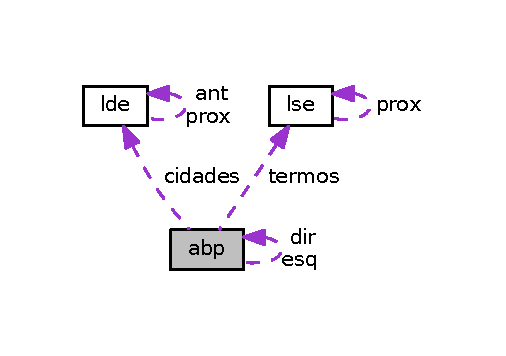
\includegraphics[width=243pt]{structabp__coll__graph}
\end{center}
\end{figure}
\subsection*{Campos de Dados}
\begin{DoxyCompactItemize}
\item 
int \hyperlink{structabp_a2ca276b8f2f9e2a163dc0d9504e846c2}{qtde\+Acessos}
\item 
int \hyperlink{structabp_aba05845525837a0260605d109242fb49}{qtde\+Termos}
\item 
\hyperlink{struct_8h_a0d3de75d86bf1db6f749c91f755b870c}{L\+SE} $\ast$ \hyperlink{structabp_a455687e406c855e366193f3ba638ed6d}{termos}
\item 
\hyperlink{struct_8h_ae030205799002e4fc414e374283d8598}{L\+DE} $\ast$ \hyperlink{structabp_ac621929c65d21c284f2897d0dc34777c}{cidades}
\item 
struct \hyperlink{structabp}{abp} $\ast$ \hyperlink{structabp_aa1052089fda0e5ed652bbe60126de869}{esq}
\item 
struct \hyperlink{structabp}{abp} $\ast$ \hyperlink{structabp_a68e9acbab0de7ab617165c904c98334f}{dir}
\end{DoxyCompactItemize}


\subsection{Descrição detalhada}
Arvore binária. 

Arvore binária de pesquisa responsável por guardar todos os dados das consultas. Cada nodo da árvore representa uma consulta, armazenando os termos da consulta, além das cidades que realizaram essa consulta.

\begin{DoxyWarning}{Aviso}
A árvore é binária de pesquisa, P\+O\+RÉM a chave dela não é tão útil para a realização das pesquisas. 
\end{DoxyWarning}

\hypertarget{structdescritor}{}\section{Referência à estrutura descritor}
\label{structdescritor}\index{descritor@{descritor}}


Estrutura principal do programa, responsável por guardar T\+O\+D\+OS os dados.  




{\ttfamily \#include $<$struct.\+h$>$}



Diagrama de colaboração para descritor\+:\nopagebreak
\begin{figure}[H]
\begin{center}
\leavevmode
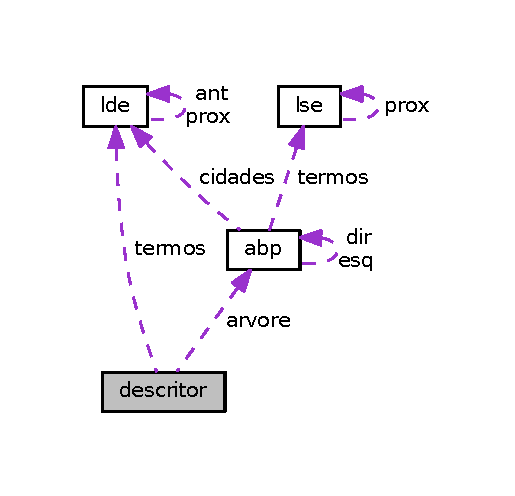
\includegraphics[width=247pt]{structdescritor__coll__graph}
\end{center}
\end{figure}
\subsection*{Campos de Dados}
\begin{DoxyCompactItemize}
\item 
\hyperlink{struct_8h_a1664119ce88635d3bf4655a988ef8248}{Consulta} $\ast$ \hyperlink{structdescritor_a523b6d27352566be093cada88aa655d4}{arvore}
\item 
\hyperlink{struct_8h_ae030205799002e4fc414e374283d8598}{L\+DE} $\ast$ \hyperlink{structdescritor_a4f74c1b0743b541ef2b21dec4fa4da2e}{termos}
\end{DoxyCompactItemize}


\subsection{Descrição detalhada}
Estrutura principal do programa, responsável por guardar T\+O\+D\+OS os dados. 

Estrutura principal do programa, que guarda tanto a árvore binária de pesquisa {\ttfamily arvore}, como a lista geral de termos consultados {\ttfamily termos}. 

\hypertarget{structlde}{}\section{Referência à estrutura lde}
\label{structlde}\index{lde@{lde}}


Lista duplamente encadeada.  




{\ttfamily \#include $<$struct.\+h$>$}



Diagrama de colaboração para lde\+:\nopagebreak
\begin{figure}[H]
\begin{center}
\leavevmode
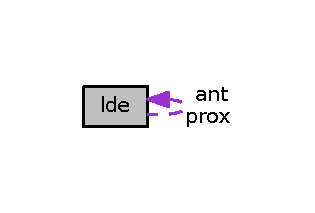
\includegraphics[width=151pt]{structlde__coll__graph}
\end{center}
\end{figure}
\subsection*{Campos de Dados}
\begin{DoxyCompactItemize}
\item 
char \hyperlink{structlde_aa4e90ca99702bac9e1c78503ad86acba}{nome} \mbox{[}100\mbox{]}
\item 
int \hyperlink{structlde_aa8a45bf920d47706309cd931134d5219}{qtde}
\item 
struct \hyperlink{structlde}{lde} $\ast$ \hyperlink{structlde_a842cbaea6d55e782335dcad1a6992695}{prox}
\item 
struct \hyperlink{structlde}{lde} $\ast$ \hyperlink{structlde_a9533d032f1309656dcf523f30de08484}{ant}
\end{DoxyCompactItemize}


\subsection{Descrição detalhada}
Lista duplamente encadeada. 

Lista duplamente encadeada, que pode ou não ser circular. 

\subsection{Documentação dos campos e atributos}
\mbox{\Hypertarget{structlde_a9533d032f1309656dcf523f30de08484}\label{structlde_a9533d032f1309656dcf523f30de08484}} 
\index{lde@{lde}!ant@{ant}}
\index{ant@{ant}!lde@{lde}}
\subsubsection{\texorpdfstring{ant}{ant}}
{\footnotesize\ttfamily struct \hyperlink{structlde}{lde}$\ast$ ant}

Ponteiro que aponta para o elemento anterior da lista \mbox{\Hypertarget{structlde_aa4e90ca99702bac9e1c78503ad86acba}\label{structlde_aa4e90ca99702bac9e1c78503ad86acba}} 
\index{lde@{lde}!nome@{nome}}
\index{nome@{nome}!lde@{lde}}
\subsubsection{\texorpdfstring{nome}{nome}}
{\footnotesize\ttfamily char nome\mbox{[}100\mbox{]}}

String de tamanho máximo 100 \mbox{\Hypertarget{structlde_a842cbaea6d55e782335dcad1a6992695}\label{structlde_a842cbaea6d55e782335dcad1a6992695}} 
\index{lde@{lde}!prox@{prox}}
\index{prox@{prox}!lde@{lde}}
\subsubsection{\texorpdfstring{prox}{prox}}
{\footnotesize\ttfamily struct \hyperlink{structlde}{lde}$\ast$ prox}

Ponteiro que aponta para o próximo elemento da lista \mbox{\Hypertarget{structlde_aa8a45bf920d47706309cd931134d5219}\label{structlde_aa8a45bf920d47706309cd931134d5219}} 
\index{lde@{lde}!qtde@{qtde}}
\index{qtde@{qtde}!lde@{lde}}
\subsubsection{\texorpdfstring{qtde}{qtde}}
{\footnotesize\ttfamily int qtde}

Inteiro que armazena quantas vezes esse nodo foi acessado e/ou chamado e/ou requisitado 

A documentação para esta estrutura foi gerada a partir do seguinte ficheiro\+:\begin{DoxyCompactItemize}
\item 
\hyperlink{struct_8h}{struct.\+h}\end{DoxyCompactItemize}

\hypertarget{structlse}{}\section{Referência à estrutura lse}
\label{structlse}\index{lse@{lse}}


Lista simplesmente encadeada.  




{\ttfamily \#include $<$struct.\+h$>$}



Diagrama de colaboração para lse\+:\nopagebreak
\begin{figure}[H]
\begin{center}
\leavevmode
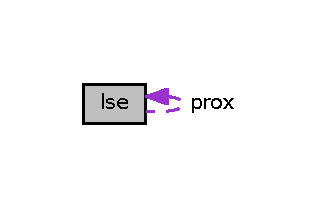
\includegraphics[width=153pt]{structlse__coll__graph}
\end{center}
\end{figure}
\subsection*{Campos de Dados}
\begin{DoxyCompactItemize}
\item 
char \hyperlink{structlse_a9df8ca8433f565cd387dd62ce6023a51}{termo} \mbox{[}100\mbox{]}
\item 
struct \hyperlink{structlse}{lse} $\ast$ \hyperlink{structlse_af49f0d9ba8c6fde74ac1b0ffef3c992b}{prox}
\end{DoxyCompactItemize}


\subsection{Descrição detalhada}
Lista simplesmente encadeada. 

\subsection{Documentação dos campos e atributos}
\mbox{\Hypertarget{structlse_af49f0d9ba8c6fde74ac1b0ffef3c992b}\label{structlse_af49f0d9ba8c6fde74ac1b0ffef3c992b}} 
\index{lse@{lse}!prox@{prox}}
\index{prox@{prox}!lse@{lse}}
\subsubsection{\texorpdfstring{prox}{prox}}
{\footnotesize\ttfamily struct \hyperlink{structlse}{lse}$\ast$ prox}

Ponteiro que aponta para o próximo elemento da lista \mbox{\Hypertarget{structlse_a9df8ca8433f565cd387dd62ce6023a51}\label{structlse_a9df8ca8433f565cd387dd62ce6023a51}} 
\index{lse@{lse}!termo@{termo}}
\index{termo@{termo}!lse@{lse}}
\subsubsection{\texorpdfstring{termo}{termo}}
{\footnotesize\ttfamily char termo\mbox{[}100\mbox{]}}

String de tamanho máximo 100 

A documentação para esta estrutura foi gerada a partir do seguinte ficheiro\+:\begin{DoxyCompactItemize}
\item 
\hyperlink{struct_8h}{struct.\+h}\end{DoxyCompactItemize}

\hypertarget{structs__qtd_cons}{}\section{Referência à estrutura s\+\_\+qtd\+Cons}
\label{structs__qtd_cons}\index{s\+\_\+qtd\+Cons@{s\+\_\+qtd\+Cons}}


Estrutura utilizada para guardar uma L\+SE e um valor numérico arbitrário.  




{\ttfamily \#include $<$struct.\+h$>$}



Diagrama de colaboração para s\+\_\+qtd\+Cons\+:\nopagebreak
\begin{figure}[H]
\begin{center}
\leavevmode
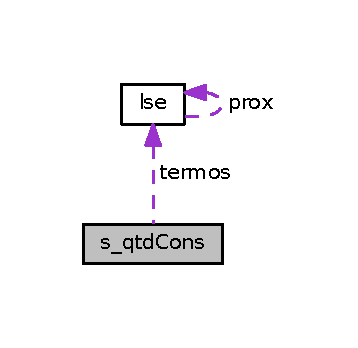
\includegraphics[width=172pt]{structs__qtd_cons__coll__graph}
\end{center}
\end{figure}
\subsection*{Campos de Dados}
\begin{DoxyCompactItemize}
\item 
\mbox{\Hypertarget{structs__qtd_cons_ab64e355d6f14927f41266ddfbf88ac91}\label{structs__qtd_cons_ab64e355d6f14927f41266ddfbf88ac91}} 
int {\bfseries qtd}
\item 
\mbox{\Hypertarget{structs__qtd_cons_a455687e406c855e366193f3ba638ed6d}\label{structs__qtd_cons_a455687e406c855e366193f3ba638ed6d}} 
\hyperlink{struct_8h_a0d3de75d86bf1db6f749c91f755b870c}{L\+SE} $\ast$ {\bfseries termos}
\end{DoxyCompactItemize}


\subsection{Descrição detalhada}
Estrutura utilizada para guardar uma L\+SE e um valor numérico arbitrário. 

Estrutura que é utilizada somente na função \hyperlink{operacoes_8h_a51685935591ec37d31c3a5600fe3f721}{consultas\+Por\+Localidade()} para poder armazenar quantas vezes uma {\ttfamily L\+S\+E$\ast$} foi chamada. 

A documentação para esta estrutura foi gerada a partir do seguinte ficheiro\+:\begin{DoxyCompactItemize}
\item 
\hyperlink{struct_8h}{struct.\+h}\end{DoxyCompactItemize}

\chapter{Documentação dos Arquivos e Funções}
\hypertarget{arvore_8h}{}\section{Referência ao ficheiro arvore.\+h}
\label{arvore_8h}\index{arvore.\+h@{arvore.\+h}}


Arquivo que contém funções relacionadas a manipulação de dados em arvores.  


{\ttfamily \#include \char`\"{}struct.\+h\char`\"{}}\newline
Diagrama de dependências de inclusão para arvore.\+h\+:\nopagebreak
\begin{figure}[H]
\begin{center}
\leavevmode
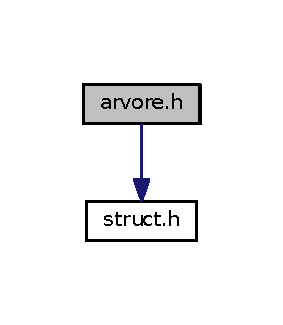
\includegraphics[width=136pt]{arvore_8h__incl}
\end{center}
\end{figure}
Este grafo mostra quais são os ficheiros que incluem directamente ou indirectamente este ficheiro\+:\nopagebreak
\begin{figure}[H]
\begin{center}
\leavevmode
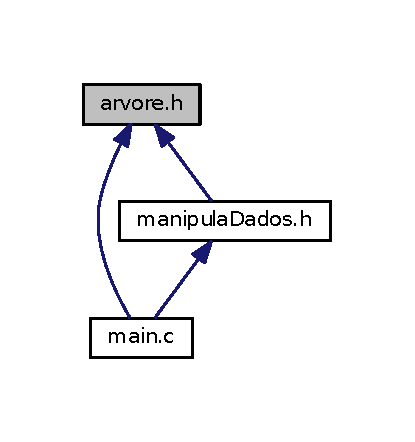
\includegraphics[width=199pt]{arvore_8h__dep__incl}
\end{center}
\end{figure}
\subsection*{Macros}
\begin{DoxyCompactItemize}
\item 
\mbox{\Hypertarget{arvore_8h_ae96f9f744c128760057a81b62848b43a}\label{arvore_8h_ae96f9f744c128760057a81b62848b43a}} 
\#define {\bfseries Q\+T\+D\+\_\+\+T\+E\+R\+M\+OS}~1
\item 
\mbox{\Hypertarget{arvore_8h_a0b936c34e70da9e8b744011a6b0ec96a}\label{arvore_8h_a0b936c34e70da9e8b744011a6b0ec96a}} 
\#define {\bfseries Q\+T\+D\+\_\+\+A\+C\+E\+S\+S\+OS}~2
\end{DoxyCompactItemize}
\subsection*{Funções}
\begin{DoxyCompactItemize}
\item 
\hyperlink{struct_8h_a1664119ce88635d3bf4655a988ef8248}{Consulta} $\ast$ \hyperlink{arvore_8h_a3c7a20806dec140adf9462f60415012f}{cria\+Arvore} ()
\begin{DoxyCompactList}\small\item\em Cria árvore. \end{DoxyCompactList}\item 
\hyperlink{struct_8h_a1664119ce88635d3bf4655a988ef8248}{Consulta} $\ast$ \hyperlink{arvore_8h_a78da70932bd92e6ffa4af27cb59690f9}{insere\+Nodo\+Arvore} (\hyperlink{struct_8h_a1664119ce88635d3bf4655a988ef8248}{Consulta} $\ast$arvore, \hyperlink{struct_8h_a0d3de75d86bf1db6f749c91f755b870c}{L\+SE} $\ast$lista\+Termos, int qtd\+Termos, char $\ast$cidade)
\begin{DoxyCompactList}\small\item\em Insere um nodo na árvore. \end{DoxyCompactList}\item 
int \hyperlink{arvore_8h_a2216ac9a9960b66516e537015a3f26f7}{percorre\+Arvore} (\hyperlink{struct_8h_a1664119ce88635d3bf4655a988ef8248}{Consulta} $\ast$nodo, int nivel)
\begin{DoxyCompactList}\small\item\em Logging de informações sobre uma árvore. \end{DoxyCompactList}\end{DoxyCompactItemize}


\subsection{Descrição detalhada}
Arquivo que contém funções relacionadas a manipulação de dados em arvores. 

\mbox{\Hypertarget{arvore_8h_a3c7a20806dec140adf9462f60415012f}\label{arvore_8h_a3c7a20806dec140adf9462f60415012f}} 
\index{arvore.\+h@{arvore.\+h}!cria\+Arvore@{cria\+Arvore}}
\index{cria\+Arvore@{cria\+Arvore}!arvore.\+h@{arvore.\+h}}
\subsubsection{\texorpdfstring{cria\+Arvore()}{criaArvore()}}
{\footnotesize\ttfamily \hyperlink{struct_8h_a1664119ce88635d3bf4655a988ef8248}{Consulta}$\ast$ cria\+Arvore (\begin{DoxyParamCaption}{ }\end{DoxyParamCaption})}



Cria árvore. 

A função \hyperlink{arvore_8h_a3c7a20806dec140adf9462f60415012f}{cria\+Arvore()} cria uma arvore vazia. \begin{DoxyReturn}{Retorna}
{\ttfamily N\+U\+LL} sempre é retornado. 
\end{DoxyReturn}
Este é o diagrama das funções que utilizam esta função\+:\nopagebreak
\begin{figure}[H]
\begin{center}
\leavevmode
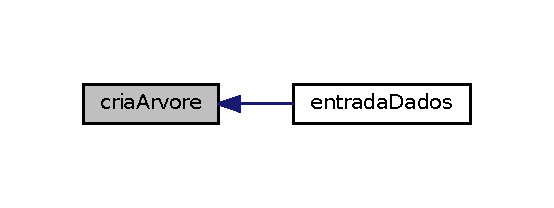
\includegraphics[width=266pt]{arvore_8h_a3c7a20806dec140adf9462f60415012f_icgraph}
\end{center}
\end{figure}
\mbox{\Hypertarget{arvore_8h_a78da70932bd92e6ffa4af27cb59690f9}\label{arvore_8h_a78da70932bd92e6ffa4af27cb59690f9}} 
\index{arvore.\+h@{arvore.\+h}!insere\+Nodo\+Arvore@{insere\+Nodo\+Arvore}}
\index{insere\+Nodo\+Arvore@{insere\+Nodo\+Arvore}!arvore.\+h@{arvore.\+h}}
\subsubsection{\texorpdfstring{insere\+Nodo\+Arvore()}{insereNodoArvore()}}
{\footnotesize\ttfamily \hyperlink{struct_8h_a1664119ce88635d3bf4655a988ef8248}{Consulta}$\ast$ insere\+Nodo\+Arvore (\begin{DoxyParamCaption}\item[{\hyperlink{struct_8h_a1664119ce88635d3bf4655a988ef8248}{Consulta} $\ast$}]{arvore,  }\item[{\hyperlink{struct_8h_a0d3de75d86bf1db6f749c91f755b870c}{L\+SE} $\ast$}]{lista\+Termos,  }\item[{int}]{qtd\+Termos,  }\item[{char $\ast$}]{cidade }\end{DoxyParamCaption})}



Insere um nodo na árvore. 

A função \hyperlink{arvore_8h_a78da70932bd92e6ffa4af27cb59690f9}{insere\+Nodo\+Arvore()} é responsável por inserir um nodo na árvore (ou incrementar ou contador, caso o nodo já exista) 
\begin{DoxyParams}{Parâmetros}
{\em arvore} & Árvore na qual será inserido o novo nodo \\
\hline
{\em lista\+Termos} & Lista dos termos que esse novo nodo irá conter (consulta) \\
\hline
{\em qtd\+Termos} & Tamanho da {\ttfamily lista\+Termos} \\
\hline
{\em cidade} & String com o nome da cidade na qual foi realizada a consulta \\
\hline
\end{DoxyParams}
\begin{DoxyReturn}{Retorna}
{\ttfamily $\ast$\+Consulta} contendo a arvore recebida, com a adição/incrementação do novo nodo. 
\end{DoxyReturn}
Grafo de chamadas desta função\+:\nopagebreak
\begin{figure}[H]
\begin{center}
\leavevmode
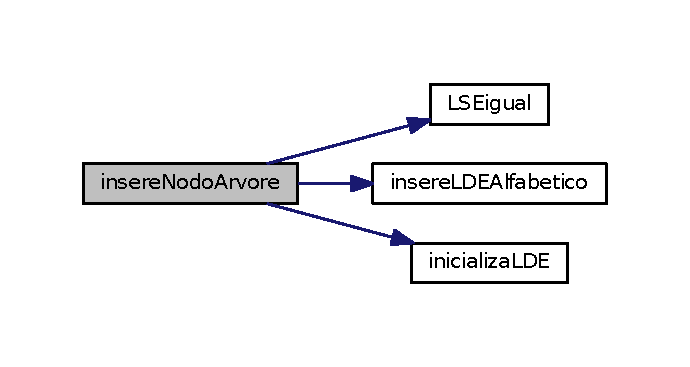
\includegraphics[width=331pt]{arvore_8h_a78da70932bd92e6ffa4af27cb59690f9_cgraph}
\end{center}
\end{figure}
Este é o diagrama das funções que utilizam esta função\+:\nopagebreak
\begin{figure}[H]
\begin{center}
\leavevmode
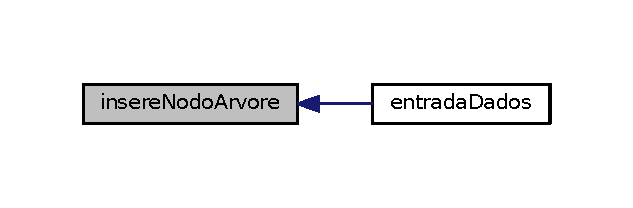
\includegraphics[width=304pt]{arvore_8h_a78da70932bd92e6ffa4af27cb59690f9_icgraph}
\end{center}
\end{figure}
\mbox{\Hypertarget{arvore_8h_a2216ac9a9960b66516e537015a3f26f7}\label{arvore_8h_a2216ac9a9960b66516e537015a3f26f7}} 
\index{arvore.\+h@{arvore.\+h}!percorre\+Arvore@{percorre\+Arvore}}
\index{percorre\+Arvore@{percorre\+Arvore}!arvore.\+h@{arvore.\+h}}
\subsubsection{\texorpdfstring{percorre\+Arvore()}{percorreArvore()}}
{\footnotesize\ttfamily int percorre\+Arvore (\begin{DoxyParamCaption}\item[{\hyperlink{struct_8h_a1664119ce88635d3bf4655a988ef8248}{Consulta} $\ast$}]{nodo,  }\item[{int}]{nivel }\end{DoxyParamCaption})}



Logging de informações sobre uma árvore. 

A função \hyperlink{arvore_8h_a2216ac9a9960b66516e537015a3f26f7}{percorre\+Arvore()} é responsável por printar na tela do terminal, informações a respeito de cada nodo da árvore 
\begin{DoxyParams}{Parâmetros}
{\em nodo} & Nodo inicial da árvore \\
\hline
{\em nivel} & Valor inicial para o nível da árvore (Para satisfazer ambas convenções de nível inicial = 0 ou 1)\\
\hline
\end{DoxyParams}
\begin{DoxyReturn}{Retorna}
Altura da arvore -\/ 1 + {\ttfamily nivel} 
\end{DoxyReturn}
Grafo de chamadas desta função\+:\nopagebreak
\begin{figure}[H]
\begin{center}
\leavevmode
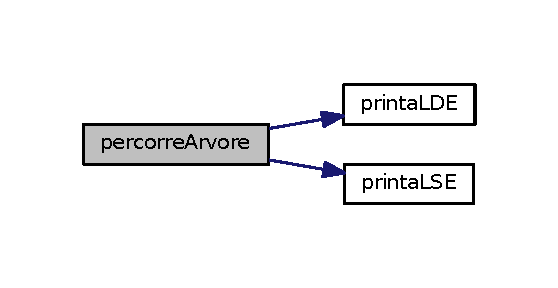
\includegraphics[width=268pt]{arvore_8h_a2216ac9a9960b66516e537015a3f26f7_cgraph}
\end{center}
\end{figure}

\hypertarget{benchmark_8h}{}\section{Referência ao ficheiro benchmark.\+h}
\label{benchmark_8h}\index{benchmark.\+h@{benchmark.\+h}}


Arquivo que contém funções relacionadas a medição do tempo gasto para realizar as operações de entrada//saida de dados.  


{\ttfamily \#include \char`\"{}struct.\+h\char`\"{}}\newline
Diagrama de dependências de inclusão para benchmark.\+h\+:\nopagebreak
\begin{figure}[H]
\begin{center}
\leavevmode
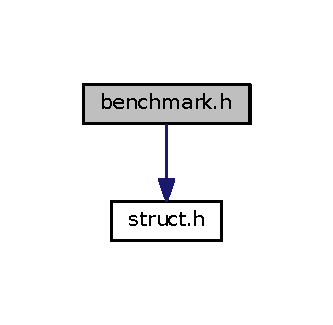
\includegraphics[width=160pt]{benchmark_8h__incl}
\end{center}
\end{figure}
Este grafo mostra quais são os ficheiros que incluem directamente ou indirectamente este ficheiro\+:\nopagebreak
\begin{figure}[H]
\begin{center}
\leavevmode
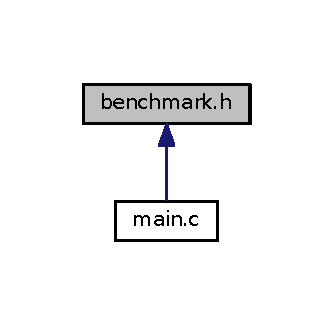
\includegraphics[width=160pt]{benchmark_8h__dep__incl}
\end{center}
\end{figure}
\subsection*{Funções}
\begin{DoxyCompactItemize}
\item 
\hyperlink{struct_8h_a1f5d65da7c19674431ada6dcf434b9ec}{Info} $\ast$ \hyperlink{benchmark_8h_a052cafc2d6cd429354bf898787b124c5}{info\+Benchmark} (\hyperlink{struct_8h_a1f5d65da7c19674431ada6dcf434b9ec}{Info} $\ast$($\ast$function)(F\+I\+LE $\ast$), F\+I\+LE $\ast$entrada)
\begin{DoxyCompactList}\small\item\em Benchmark da entrada de dados. \end{DoxyCompactList}\item 
void \hyperlink{benchmark_8h_ac01505244d5cb5d97b243b11d79be624}{operacoes\+Benchmark} (int($\ast$function)(F\+I\+LE $\ast$, F\+I\+LE $\ast$, \hyperlink{struct_8h_a1f5d65da7c19674431ada6dcf434b9ec}{Info} $\ast$), F\+I\+LE $\ast$operacoes, F\+I\+LE $\ast$saida, \hyperlink{struct_8h_a1f5d65da7c19674431ada6dcf434b9ec}{Info} $\ast$dados)
\begin{DoxyCompactList}\small\item\em Benchmark da saida de dados. \end{DoxyCompactList}\end{DoxyCompactItemize}


\subsection{Descrição detalhada}
Arquivo que contém funções relacionadas a medição do tempo gasto para realizar as operações de entrada//saida de dados. 

\mbox{\Hypertarget{benchmark_8h_a052cafc2d6cd429354bf898787b124c5}\label{benchmark_8h_a052cafc2d6cd429354bf898787b124c5}} 
\index{benchmark.\+h@{benchmark.\+h}!info\+Benchmark@{info\+Benchmark}}
\index{info\+Benchmark@{info\+Benchmark}!benchmark.\+h@{benchmark.\+h}}
\subsubsection{\texorpdfstring{info\+Benchmark()}{infoBenchmark()}}
{\footnotesize\ttfamily \hyperlink{struct_8h_a1f5d65da7c19674431ada6dcf434b9ec}{Info}$\ast$ info\+Benchmark (\begin{DoxyParamCaption}\item[{\hyperlink{struct_8h_a1f5d65da7c19674431ada6dcf434b9ec}{Info} $\ast$($\ast$)(F\+I\+LE $\ast$)}]{function,  }\item[{F\+I\+LE $\ast$}]{entrada }\end{DoxyParamCaption})}



Benchmark da entrada de dados. 

A função \hyperlink{benchmark_8h_a052cafc2d6cd429354bf898787b124c5}{info\+Benchmark()} é responsável pela medição do tempo que a função {\ttfamily function} demora para realizar a inserção dos dados na estrutura.


\begin{DoxyParams}{Parâmetros}
{\em function} & Função da qual será medido o tempo. O\+BS.\+: Ela precisa ser do tipo {\ttfamily Info$\ast$}, e receber como parâmetro {\ttfamily F\+I\+L\+E$\ast$} \\
\hline
{\em entrada} & Arquivo que contém os dados de entrada. Será passado como parâmetro para {\ttfamily function}.\\
\hline
\end{DoxyParams}
\begin{DoxyReturn}{Retorna}
{\ttfamily Info$\ast$} que é o mesmo que é retornado por {\ttfamily function}. 
\end{DoxyReturn}
\mbox{\Hypertarget{benchmark_8h_ac01505244d5cb5d97b243b11d79be624}\label{benchmark_8h_ac01505244d5cb5d97b243b11d79be624}} 
\index{benchmark.\+h@{benchmark.\+h}!operacoes\+Benchmark@{operacoes\+Benchmark}}
\index{operacoes\+Benchmark@{operacoes\+Benchmark}!benchmark.\+h@{benchmark.\+h}}
\subsubsection{\texorpdfstring{operacoes\+Benchmark()}{operacoesBenchmark()}}
{\footnotesize\ttfamily void operacoes\+Benchmark (\begin{DoxyParamCaption}\item[{int($\ast$)(F\+I\+LE $\ast$, F\+I\+LE $\ast$, \hyperlink{struct_8h_a1f5d65da7c19674431ada6dcf434b9ec}{Info} $\ast$)}]{function,  }\item[{F\+I\+LE $\ast$}]{operacoes,  }\item[{F\+I\+LE $\ast$}]{saida,  }\item[{\hyperlink{struct_8h_a1f5d65da7c19674431ada6dcf434b9ec}{Info} $\ast$}]{dados }\end{DoxyParamCaption})}



Benchmark da saida de dados. 

A função \hyperlink{benchmark_8h_ac01505244d5cb5d97b243b11d79be624}{operacoes\+Benchmark()} é responsável pela medição do tempo que a função {\ttfamily function} demora para realizar as operações e escrever a saída dos dados em um arquivo.


\begin{DoxyParams}{Parâmetros}
{\em function} & Função da qual será medido o tempo. O\+BS.\+: Ela precisa ser do tipo {\ttfamily int}, e receber como parâmetro $<$F\+I\+L\+E$\ast$, F\+I\+L\+E$\ast$, Info$\ast$$>$ \\
\hline
{\em operacoes} & Arquivo que contém os dados das operações a serem realizadas em {\ttfamily dados}. Será passado como parâmetro para {\ttfamily function}. \\
\hline
{\em saida} & Arquivo onde serão impressos os dados de saída. Será passado como parâmetro para {\ttfamily function}. \\
\hline
{\em dados} & Dados onde serão realizadas as operações descritas em {\ttfamily operacoes}. Será passado como parâmetro para {\ttfamily function}.\\
\hline
\end{DoxyParams}
\begin{DoxyReturn}{Retorna}
{\ttfamily int} que é a quantidade de operações realizadas com sucesso. 
\end{DoxyReturn}

\hypertarget{lde_8h}{}\section{Referência ao ficheiro lde.\+h}
\label{lde_8h}\index{lde.\+h@{lde.\+h}}


Arquivo que contém funções relacionadas a manipulação de listas duplamente encadeadas.  


{\ttfamily \#include \char`\"{}struct.\+h\char`\"{}}\newline
{\ttfamily \#include $<$stdio.\+h$>$}\newline
Diagrama de dependências de inclusão para lde.\+h\+:\nopagebreak
\begin{figure}[H]
\begin{center}
\leavevmode
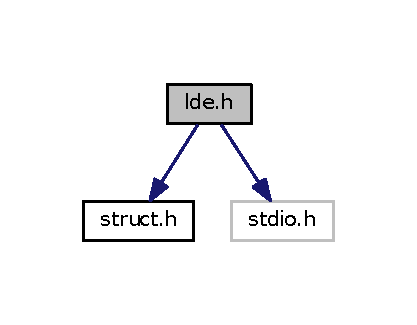
\includegraphics[width=200pt]{lde_8h__incl}
\end{center}
\end{figure}
Este grafo mostra quais são os ficheiros que incluem directamente ou indirectamente este ficheiro\+:\nopagebreak
\begin{figure}[H]
\begin{center}
\leavevmode
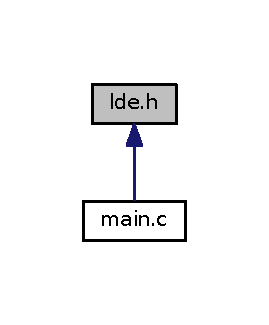
\includegraphics[width=129pt]{lde_8h__dep__incl}
\end{center}
\end{figure}
\subsection*{Funções}
\begin{DoxyCompactItemize}
\item 
\hyperlink{struct_8h_ae030205799002e4fc414e374283d8598}{L\+DE} $\ast$ \hyperlink{lde_8h_abf1ed757950e3e4965ad96d64b2aee67}{inicializa\+L\+DE} ()
\begin{DoxyCompactList}\small\item\em Cria uma lista duplamente encadeada. \end{DoxyCompactList}\item 
\hyperlink{struct_8h_ae030205799002e4fc414e374283d8598}{L\+DE} $\ast$ \hyperlink{lde_8h_ae3e979b91f4e13e245b774c4c04a4e20}{insere\+L\+D\+E\+Alfabetico} (\hyperlink{struct_8h_ae030205799002e4fc414e374283d8598}{L\+DE} $\ast$lista, char $\ast$nome)
\begin{DoxyCompactList}\small\item\em Insere um item na L\+DE, deixando-\/a em ordem alfabética. \end{DoxyCompactList}\item 
\hyperlink{struct_8h_ae030205799002e4fc414e374283d8598}{L\+DE} $\ast$ \hyperlink{lde_8h_a695bd097eab9845e2eddd196523c58ac}{insere\+L\+D\+E\+Numerico} (\hyperlink{struct_8h_ae030205799002e4fc414e374283d8598}{L\+DE} $\ast$lista, char $\ast$nome, int qtde)
\begin{DoxyCompactList}\small\item\em Insere um item na L\+DE, deixando-\/a em ordem numérica. \end{DoxyCompactList}\item 
void \hyperlink{lde_8h_a2367200509bfed169f74596bdc08cc33}{printa\+L\+DE} (\hyperlink{struct_8h_ae030205799002e4fc414e374283d8598}{L\+DE} $\ast$lista, int qtde, F\+I\+LE $\ast$saida)
\begin{DoxyCompactList}\small\item\em Logging de informações sobre a lista. \end{DoxyCompactList}\end{DoxyCompactItemize}


\subsection{Descrição detalhada}
Arquivo que contém funções relacionadas a manipulação de listas duplamente encadeadas. 

\mbox{\Hypertarget{lde_8h_abf1ed757950e3e4965ad96d64b2aee67}\label{lde_8h_abf1ed757950e3e4965ad96d64b2aee67}} 
\index{lde.\+h@{lde.\+h}!inicializa\+L\+DE@{inicializa\+L\+DE}}
\index{inicializa\+L\+DE@{inicializa\+L\+DE}!lde.\+h@{lde.\+h}}
\subsubsection{\texorpdfstring{inicializa\+L\+D\+E()}{inicializaLDE()}}
{\footnotesize\ttfamily \hyperlink{struct_8h_ae030205799002e4fc414e374283d8598}{L\+DE}$\ast$ inicializa\+L\+DE (\begin{DoxyParamCaption}{ }\end{DoxyParamCaption})}



Cria uma lista duplamente encadeada. 

A função \hyperlink{lde_8h_abf1ed757950e3e4965ad96d64b2aee67}{inicializa\+L\+D\+E()} cria uma lista duplamente encadeada vazia. \begin{DoxyReturn}{Retorna}
{\ttfamily N\+U\+LL} sempre é retornado. 
\end{DoxyReturn}
Este é o diagrama das funções que utilizam esta função\+:\nopagebreak
\begin{figure}[H]
\begin{center}
\leavevmode
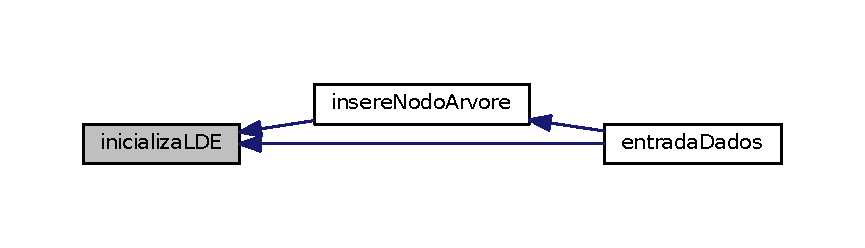
\includegraphics[width=350pt]{lde_8h_abf1ed757950e3e4965ad96d64b2aee67_icgraph}
\end{center}
\end{figure}
\mbox{\Hypertarget{lde_8h_ae3e979b91f4e13e245b774c4c04a4e20}\label{lde_8h_ae3e979b91f4e13e245b774c4c04a4e20}} 
\index{lde.\+h@{lde.\+h}!insere\+L\+D\+E\+Alfabetico@{insere\+L\+D\+E\+Alfabetico}}
\index{insere\+L\+D\+E\+Alfabetico@{insere\+L\+D\+E\+Alfabetico}!lde.\+h@{lde.\+h}}
\subsubsection{\texorpdfstring{insere\+L\+D\+E\+Alfabetico()}{insereLDEAlfabetico()}}
{\footnotesize\ttfamily \hyperlink{struct_8h_ae030205799002e4fc414e374283d8598}{L\+DE}$\ast$ insere\+L\+D\+E\+Alfabetico (\begin{DoxyParamCaption}\item[{\hyperlink{struct_8h_ae030205799002e4fc414e374283d8598}{L\+DE} $\ast$}]{lista,  }\item[{char $\ast$}]{nome }\end{DoxyParamCaption})}



Insere um item na L\+DE, deixando-\/a em ordem alfabética. 

A função \hyperlink{lde_8h_ae3e979b91f4e13e245b774c4c04a4e20}{insere\+L\+D\+E\+Alfabetico()} é responsável por inserir um item na L\+DE, fazendo que com a L\+DE sempre fique em ordem alfabética. Caso um item seja igual a algum que já está inserido, é incrementado um contador, mostrando que aquele termo foi inserido mais de uma vez. 
\begin{DoxyParams}{Parâmetros}
{\em lista} & Lista Duplamente Encadeada na qual será inserido o novo item \\
\hline
{\em nome} & String contendo o item que será inserido na lista\\
\hline
\end{DoxyParams}
\begin{DoxyReturn}{Retorna}
{\ttfamily $\ast$\+L\+DE} contendo a lista recebida, com a adição/incrementação do novo item. 
\end{DoxyReturn}
Este é o diagrama das funções que utilizam esta função\+:\nopagebreak
\begin{figure}[H]
\begin{center}
\leavevmode
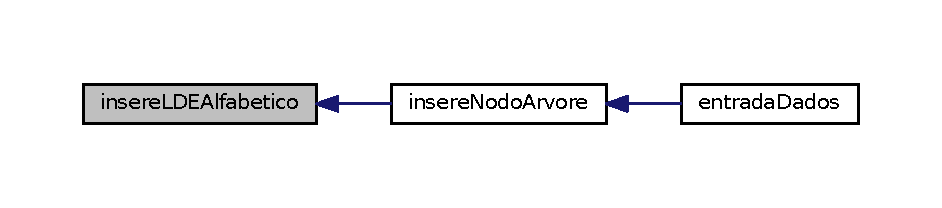
\includegraphics[width=350pt]{lde_8h_ae3e979b91f4e13e245b774c4c04a4e20_icgraph}
\end{center}
\end{figure}
\mbox{\Hypertarget{lde_8h_a695bd097eab9845e2eddd196523c58ac}\label{lde_8h_a695bd097eab9845e2eddd196523c58ac}} 
\index{lde.\+h@{lde.\+h}!insere\+L\+D\+E\+Numerico@{insere\+L\+D\+E\+Numerico}}
\index{insere\+L\+D\+E\+Numerico@{insere\+L\+D\+E\+Numerico}!lde.\+h@{lde.\+h}}
\subsubsection{\texorpdfstring{insere\+L\+D\+E\+Numerico()}{insereLDENumerico()}}
{\footnotesize\ttfamily \hyperlink{struct_8h_ae030205799002e4fc414e374283d8598}{L\+DE}$\ast$ insere\+L\+D\+E\+Numerico (\begin{DoxyParamCaption}\item[{\hyperlink{struct_8h_ae030205799002e4fc414e374283d8598}{L\+DE} $\ast$}]{lista,  }\item[{char $\ast$}]{nome,  }\item[{int}]{qtde }\end{DoxyParamCaption})}



Insere um item na L\+DE, deixando-\/a em ordem numérica. 

A função \hyperlink{lde_8h_a695bd097eab9845e2eddd196523c58ac}{insere\+L\+D\+E\+Numerico()} é responsável por inserir um item na L\+DE, fazendo que com a L\+DE sempre fique em ordem numérica decrescente. Caso um item tenha o mesmo valor numérico que outro, eles são ordenados de forma alfabética. Caso um item com a mesma quantidade numérica e tenha seu nome igual a algum que já está inserido, é incrementado um contador, mostrando que aquele termo foi inserido mais de uma vez. 
\begin{DoxyParams}{Parâmetros}
{\em lista} & Lista Duplamente Encadeada na qual será inserido o novo item \\
\hline
{\em nome} & String contendo o item que será inserido na lista \\
\hline
{\em qtde} & Numero que representa a quantidade de vezes que ele foi chamado. \\
\hline
\end{DoxyParams}
\begin{DoxyReturn}{Retorna}
{\ttfamily $\ast$\+L\+DE} contendo a lista recebida, com a adição/incrementação do novo item. 
\end{DoxyReturn}
Este é o diagrama das funções que utilizam esta função\+:\nopagebreak
\begin{figure}[H]
\begin{center}
\leavevmode
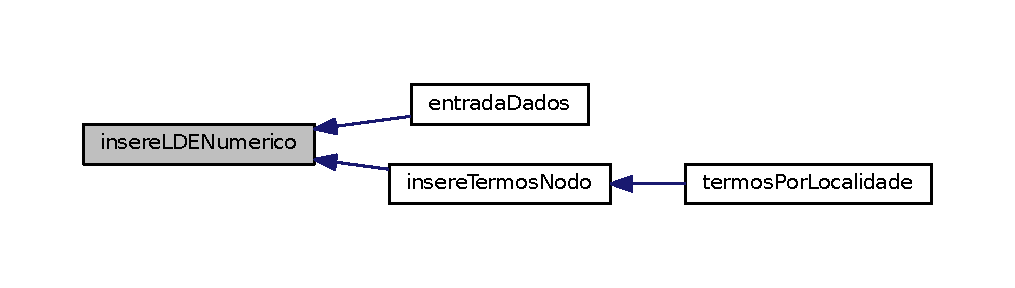
\includegraphics[width=350pt]{lde_8h_a695bd097eab9845e2eddd196523c58ac_icgraph}
\end{center}
\end{figure}
\mbox{\Hypertarget{lde_8h_a2367200509bfed169f74596bdc08cc33}\label{lde_8h_a2367200509bfed169f74596bdc08cc33}} 
\index{lde.\+h@{lde.\+h}!printa\+L\+DE@{printa\+L\+DE}}
\index{printa\+L\+DE@{printa\+L\+DE}!lde.\+h@{lde.\+h}}
\subsubsection{\texorpdfstring{printa\+L\+D\+E()}{printaLDE()}}
{\footnotesize\ttfamily void printa\+L\+DE (\begin{DoxyParamCaption}\item[{\hyperlink{struct_8h_ae030205799002e4fc414e374283d8598}{L\+DE} $\ast$}]{lista,  }\item[{int}]{qtde,  }\item[{F\+I\+LE $\ast$}]{saida }\end{DoxyParamCaption})}



Logging de informações sobre a lista. 

A função \hyperlink{lde_8h_a2367200509bfed169f74596bdc08cc33}{printa\+L\+D\+E()} é responsável por printar em um arquivo, informações a respeito de {\ttfamily qtde} itens da lista. Se o parâmetro {\ttfamily qtde} for passado como 0, a lista inteira será printada. Essa informação é printada no formato \char`\"{}@$<$qtde, nome@$>$\char`\"{}.


\begin{DoxyParams}{Parâmetros}
{\em lista} & Lista que iremos printar \\
\hline
{\em qtde} & Quantidade de termos da lista que serão printados. \\
\hline
{\em saida} & Arquivo no qual será printado a informação (pode ser passado stdout, para printar no terminal) \\
\hline
\end{DoxyParams}
Este é o diagrama das funções que utilizam esta função\+:\nopagebreak
\begin{figure}[H]
\begin{center}
\leavevmode
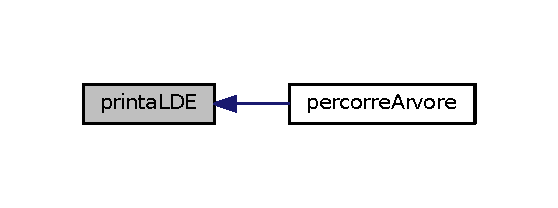
\includegraphics[width=268pt]{lde_8h_a2367200509bfed169f74596bdc08cc33_icgraph}
\end{center}
\end{figure}

\hypertarget{lse_8h}{}\section{Referência ao ficheiro lse.\+h}
\label{lse_8h}\index{lse.\+h@{lse.\+h}}


Arquivo que contém funções relacionadas a manipulação de listas simplesmente encadeadas.  


{\ttfamily \#include \char`\"{}struct.\+h\char`\"{}}\newline
Diagrama de dependências de inclusão para lse.\+h\+:\nopagebreak
\begin{figure}[H]
\begin{center}
\leavevmode
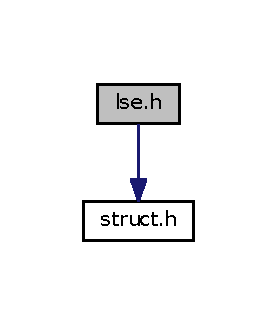
\includegraphics[width=133pt]{lse_8h__incl}
\end{center}
\end{figure}
Este grafo mostra quais são os ficheiros que incluem directamente ou indirectamente este ficheiro\+:\nopagebreak
\begin{figure}[H]
\begin{center}
\leavevmode
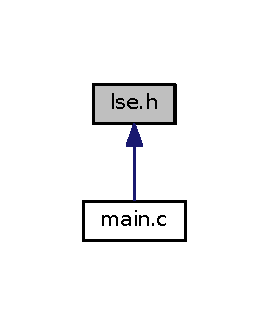
\includegraphics[width=129pt]{lse_8h__dep__incl}
\end{center}
\end{figure}
\subsection*{Funções}
\begin{DoxyCompactItemize}
\item 
\hyperlink{struct_8h_a0d3de75d86bf1db6f749c91f755b870c}{L\+SE} $\ast$ \hyperlink{lse_8h_ad765d50b06255841230e5ead220623be}{inicializa\+L\+SE} ()
\begin{DoxyCompactList}\small\item\em Cria uma lista simplesmente encadeada. \end{DoxyCompactList}\item 
\hyperlink{struct_8h_a0d3de75d86bf1db6f749c91f755b870c}{L\+SE} $\ast$ \hyperlink{lse_8h_ad004db669d206be476474b218cbb88bc}{insere\+L\+SE} (\hyperlink{struct_8h_a0d3de75d86bf1db6f749c91f755b870c}{L\+SE} $\ast$lista, char $\ast$termo)
\begin{DoxyCompactList}\small\item\em Insere um nodo em uma lista simplesmente encadeada. \end{DoxyCompactList}\item 
int \hyperlink{lse_8h_a7312566d42e1ebf660aa458dcff6338d}{L\+S\+Eigual} (\hyperlink{struct_8h_a0d3de75d86bf1db6f749c91f755b870c}{L\+SE} $\ast$lse1, \hyperlink{struct_8h_a0d3de75d86bf1db6f749c91f755b870c}{L\+SE} $\ast$lse2)
\begin{DoxyCompactList}\small\item\em Retorna 1 se duas L\+SE são identicas. \end{DoxyCompactList}\item 
void \hyperlink{lse_8h_a64b6200aec6744a6e0efb72212786248}{printa\+L\+SE} (\hyperlink{struct_8h_a0d3de75d86bf1db6f749c91f755b870c}{L\+SE} $\ast$lista, F\+I\+LE $\ast$saida)
\begin{DoxyCompactList}\small\item\em Logging de informações sobre a lista. \end{DoxyCompactList}\item 
char $\ast$ \hyperlink{lse_8h_ad18b386b8356075444b5703a7aeb4816}{parse\+L\+S\+Eto\+String} (\hyperlink{struct_8h_a0d3de75d86bf1db6f749c91f755b870c}{L\+SE} $\ast$lista, char $\ast$string)
\begin{DoxyCompactList}\small\item\em Transforma uma L\+SE em uma string. \end{DoxyCompactList}\end{DoxyCompactItemize}


\subsection{Descrição detalhada}
Arquivo que contém funções relacionadas a manipulação de listas simplesmente encadeadas. 

\begin{DoxyAuthor}{Autor}
Rafael Baldasso Audibert 

Augusto Zanella Bardini 
\end{DoxyAuthor}
\begin{DoxyDate}{Data}
11 Jul 2018 
\end{DoxyDate}


\subsection{Documentação das funções}
\mbox{\Hypertarget{lse_8h_ad765d50b06255841230e5ead220623be}\label{lse_8h_ad765d50b06255841230e5ead220623be}} 
\index{lse.\+h@{lse.\+h}!inicializa\+L\+SE@{inicializa\+L\+SE}}
\index{inicializa\+L\+SE@{inicializa\+L\+SE}!lse.\+h@{lse.\+h}}
\subsubsection{\texorpdfstring{inicializa\+L\+S\+E()}{inicializaLSE()}}
{\footnotesize\ttfamily \hyperlink{struct_8h_a0d3de75d86bf1db6f749c91f755b870c}{L\+SE}$\ast$ inicializa\+L\+SE (\begin{DoxyParamCaption}{ }\end{DoxyParamCaption})}



Cria uma lista simplesmente encadeada. 

A função \hyperlink{lse_8h_ad765d50b06255841230e5ead220623be}{inicializa\+L\+S\+E()} cria uma lista simplesmente encadeada vazia. \begin{DoxyReturn}{Retorna}
{\ttfamily N\+U\+LL} sempre é retornado. 
\end{DoxyReturn}
Este é o diagrama das funções que utilizam esta função\+:\nopagebreak
\begin{figure}[H]
\begin{center}
\leavevmode
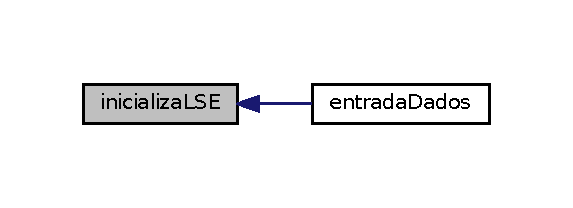
\includegraphics[width=275pt]{lse_8h_ad765d50b06255841230e5ead220623be_icgraph}
\end{center}
\end{figure}
\mbox{\Hypertarget{lse_8h_ad004db669d206be476474b218cbb88bc}\label{lse_8h_ad004db669d206be476474b218cbb88bc}} 
\index{lse.\+h@{lse.\+h}!insere\+L\+SE@{insere\+L\+SE}}
\index{insere\+L\+SE@{insere\+L\+SE}!lse.\+h@{lse.\+h}}
\subsubsection{\texorpdfstring{insere\+L\+S\+E()}{insereLSE()}}
{\footnotesize\ttfamily \hyperlink{struct_8h_a0d3de75d86bf1db6f749c91f755b870c}{L\+SE}$\ast$ insere\+L\+SE (\begin{DoxyParamCaption}\item[{\hyperlink{struct_8h_a0d3de75d86bf1db6f749c91f755b870c}{L\+SE} $\ast$}]{lista,  }\item[{char $\ast$}]{termo }\end{DoxyParamCaption})}



Insere um nodo em uma lista simplesmente encadeada. 

A função \hyperlink{lse_8h_ad004db669d206be476474b218cbb88bc}{insere\+L\+S\+E()} insere um nodo em uma lista simplesmente encadeada já existente, mantendo-\/a ordenada em ordem alfabética.


\begin{DoxyParams}{Parâmetros}
{\em lista} & Lista na qual será inserida o novo termo \\
\hline
{\em termo} & String do termo que será inserido na lista \\
\hline
\end{DoxyParams}
\begin{DoxyReturn}{Retorna}
{\ttfamily L\+S\+E$\ast$} contendo a lista recebido com a adição do novo termo. 
\end{DoxyReturn}
Este é o diagrama das funções que utilizam esta função\+:\nopagebreak
\begin{figure}[H]
\begin{center}
\leavevmode
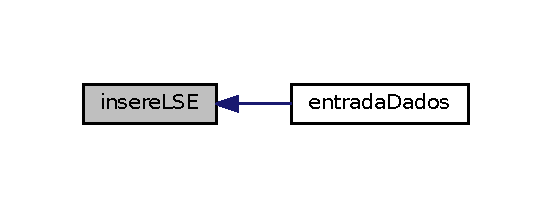
\includegraphics[width=265pt]{lse_8h_ad004db669d206be476474b218cbb88bc_icgraph}
\end{center}
\end{figure}
\mbox{\Hypertarget{lse_8h_a7312566d42e1ebf660aa458dcff6338d}\label{lse_8h_a7312566d42e1ebf660aa458dcff6338d}} 
\index{lse.\+h@{lse.\+h}!L\+S\+Eigual@{L\+S\+Eigual}}
\index{L\+S\+Eigual@{L\+S\+Eigual}!lse.\+h@{lse.\+h}}
\subsubsection{\texorpdfstring{L\+S\+Eigual()}{LSEigual()}}
{\footnotesize\ttfamily int L\+S\+Eigual (\begin{DoxyParamCaption}\item[{\hyperlink{struct_8h_a0d3de75d86bf1db6f749c91f755b870c}{L\+SE} $\ast$}]{lse1,  }\item[{\hyperlink{struct_8h_a0d3de75d86bf1db6f749c91f755b870c}{L\+SE} $\ast$}]{lse2 }\end{DoxyParamCaption})}



Retorna 1 se duas L\+SE são identicas. 

A função \hyperlink{lse_8h_a7312566d42e1ebf660aa458dcff6338d}{L\+S\+Eigual()} é responsável por dizer se {\ttfamily lse1} e {\ttfamily lse2} são idênticas.


\begin{DoxyParams}{Parâmetros}
{\em lse1} & Lista 1 \\
\hline
{\em lse2} & L\+Ista 2\\
\hline
\end{DoxyParams}
\begin{DoxyReturn}{Retorna}
{\ttfamily 1} se as listas forem idênticas, {\ttfamily 0} se as listas forem diferentes 
\end{DoxyReturn}
Este é o diagrama das funções que utilizam esta função\+:\nopagebreak
\begin{figure}[H]
\begin{center}
\leavevmode
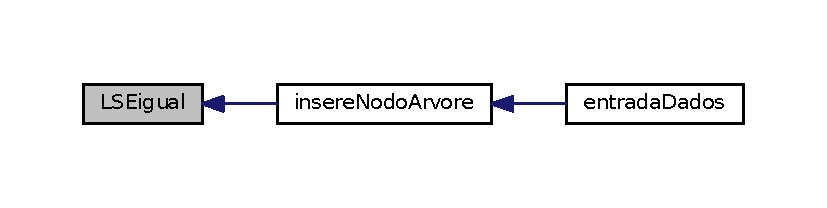
\includegraphics[width=350pt]{lse_8h_a7312566d42e1ebf660aa458dcff6338d_icgraph}
\end{center}
\end{figure}
\mbox{\Hypertarget{lse_8h_ad18b386b8356075444b5703a7aeb4816}\label{lse_8h_ad18b386b8356075444b5703a7aeb4816}} 
\index{lse.\+h@{lse.\+h}!parse\+L\+S\+Eto\+String@{parse\+L\+S\+Eto\+String}}
\index{parse\+L\+S\+Eto\+String@{parse\+L\+S\+Eto\+String}!lse.\+h@{lse.\+h}}
\subsubsection{\texorpdfstring{parse\+L\+S\+Eto\+String()}{parseLSEtoString()}}
{\footnotesize\ttfamily char$\ast$ parse\+L\+S\+Eto\+String (\begin{DoxyParamCaption}\item[{\hyperlink{struct_8h_a0d3de75d86bf1db6f749c91f755b870c}{L\+SE} $\ast$}]{lista,  }\item[{char $\ast$}]{string }\end{DoxyParamCaption})}



Transforma uma L\+SE em uma string. 

A função \hyperlink{lse_8h_ad18b386b8356075444b5703a7aeb4816}{parse\+L\+S\+Eto\+String()} é responsável por transformar uma L\+SE em uma string formatada. Seu formato é \char`\"{}\char`\"{}$<$termo; termo; termo; termo$>$".


\begin{DoxyParams}{Parâmetros}
{\em lista} & Lista que iremos transformar em string \\
\hline
{\em string} & Ponteiro para o local onde guardaremos a string\\
\hline
\end{DoxyParams}
\begin{DoxyReturn}{Retorna}
{\ttfamily $\ast$char} onde iremos guardar a string 
\end{DoxyReturn}
\begin{DoxyNote}{Nota}
Não é necessário utilizar o retorno dessa função, já que ela já recebe o ponteiro pra string na qual ela será guardada como parâmetro. Ela é retornada apenas por convenção. 
\end{DoxyNote}
\mbox{\Hypertarget{lse_8h_a64b6200aec6744a6e0efb72212786248}\label{lse_8h_a64b6200aec6744a6e0efb72212786248}} 
\index{lse.\+h@{lse.\+h}!printa\+L\+SE@{printa\+L\+SE}}
\index{printa\+L\+SE@{printa\+L\+SE}!lse.\+h@{lse.\+h}}
\subsubsection{\texorpdfstring{printa\+L\+S\+E()}{printaLSE()}}
{\footnotesize\ttfamily void printa\+L\+SE (\begin{DoxyParamCaption}\item[{\hyperlink{struct_8h_a0d3de75d86bf1db6f749c91f755b870c}{L\+SE} $\ast$}]{lista,  }\item[{F\+I\+LE $\ast$}]{saida }\end{DoxyParamCaption})}



Logging de informações sobre a lista. 

A função \hyperlink{lse_8h_a64b6200aec6744a6e0efb72212786248}{printa\+L\+S\+E()} é responsável por printar em um arquivo, informações a respeito da lista. Essa informação é printada no formato \char`\"{}@$<$termo;termo;termo;...@$>$\char`\"{}.


\begin{DoxyParams}{Parâmetros}
{\em lista} & Lista que iremos printar \\
\hline
{\em saida} & Arquivo no qual será printado a informação (pode ser passado stdout, para printar no terminal) \\
\hline
\end{DoxyParams}
Este é o diagrama das funções que utilizam esta função\+:\nopagebreak
\begin{figure}[H]
\begin{center}
\leavevmode
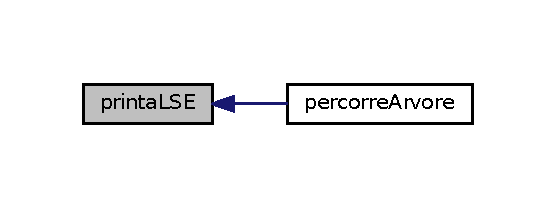
\includegraphics[width=267pt]{lse_8h_a64b6200aec6744a6e0efb72212786248_icgraph}
\end{center}
\end{figure}

\hypertarget{main_8c}{}\section{Referência ao ficheiro main.\+c}
\label{main_8c}\index{main.\+c@{main.\+c}}


Arquivo que contém a main do programa Analytics.  


{\ttfamily \#include $<$stdio.\+h$>$}\newline
{\ttfamily \#include $<$stdlib.\+h$>$}\newline
{\ttfamily \#include $<$locale.\+h$>$}\newline
{\ttfamily \#include \char`\"{}struct.\+h\char`\"{}}\newline
{\ttfamily \#include \char`\"{}manipula\+String.\+h\char`\"{}}\newline
{\ttfamily \#include \char`\"{}arvore.\+h\char`\"{}}\newline
{\ttfamily \#include \char`\"{}lse.\+h\char`\"{}}\newline
{\ttfamily \#include \char`\"{}manipula\+Dados.\+h\char`\"{}}\newline
{\ttfamily \#include \char`\"{}lde.\+h\char`\"{}}\newline
{\ttfamily \#include \char`\"{}benchmark.\+h\char`\"{}}\newline
Diagrama de dependências de inclusão para main.\+c\+:\nopagebreak
\begin{figure}[H]
\begin{center}
\leavevmode
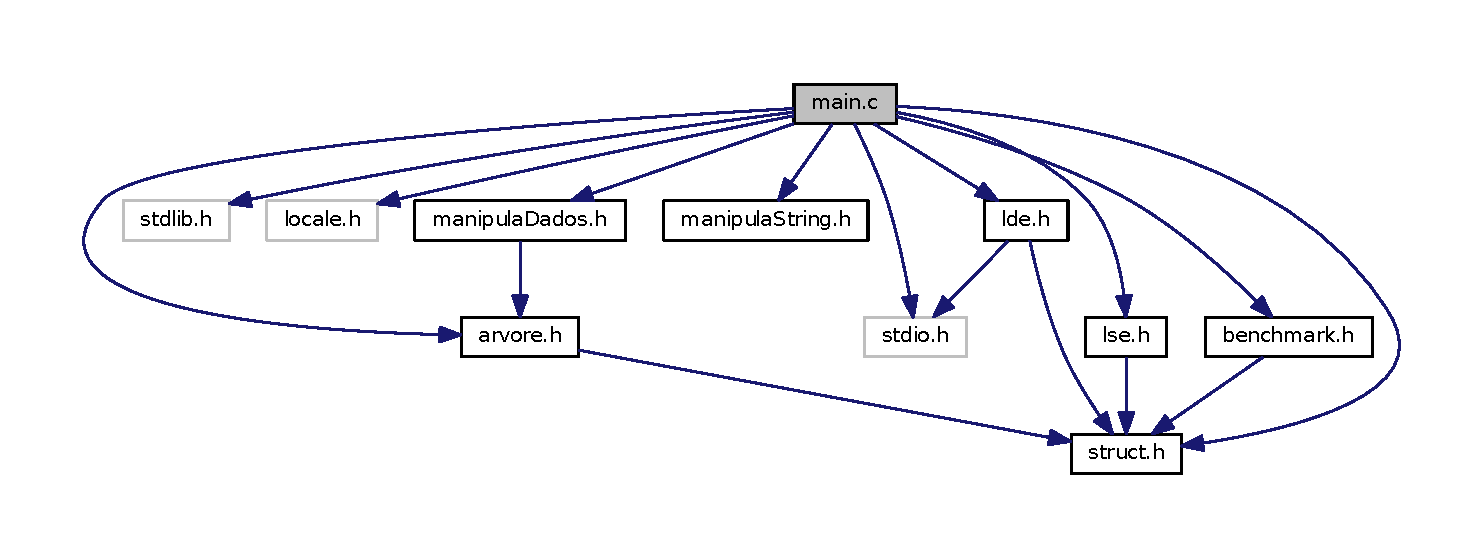
\includegraphics[width=350pt]{main_8c__incl}
\end{center}
\end{figure}
\subsection*{Macros}
\begin{DoxyCompactItemize}
\item 
\mbox{\Hypertarget{main_8c_a373f33e1065de00a8bccb33931ab2d1c}\label{main_8c_a373f33e1065de00a8bccb33931ab2d1c}} 
\#define {\bfseries F\+\_\+\+E\+N\+T\+R\+A\+DA}~\char`\"{}data/input.\+txt\char`\"{}
\item 
\mbox{\Hypertarget{main_8c_a2141ff885712fa75f5e08e769e3385d8}\label{main_8c_a2141ff885712fa75f5e08e769e3385d8}} 
\#define {\bfseries F\+\_\+\+O\+P\+E\+R\+A\+C\+O\+ES}~\char`\"{}data/operations.\+txt\char`\"{}
\item 
\mbox{\Hypertarget{main_8c_a650a755126cacd1b97fc7d5813ea9cbb}\label{main_8c_a650a755126cacd1b97fc7d5813ea9cbb}} 
\#define {\bfseries F\+\_\+\+S\+A\+I\+DA}~\char`\"{}data/saida.\+txt\char`\"{}
\end{DoxyCompactItemize}
\subsection*{Funções}
\begin{DoxyCompactItemize}
\item 
int \hyperlink{main_8c_a3c04138a5bfe5d72780bb7e82a18e627}{main} (int argc, char $\ast$$\ast$argv)
\begin{DoxyCompactList}\small\item\em Função main do programa Analytics. \end{DoxyCompactList}\end{DoxyCompactItemize}


\subsection{Descrição detalhada}
Arquivo que contém a main do programa Analytics. 

\mbox{\Hypertarget{main_8c_a3c04138a5bfe5d72780bb7e82a18e627}\label{main_8c_a3c04138a5bfe5d72780bb7e82a18e627}} 
\index{main.\+c@{main.\+c}!main@{main}}
\index{main@{main}!main.\+c@{main.\+c}}
\subsubsection{\texorpdfstring{main()}{main()}}
{\footnotesize\ttfamily int main (\begin{DoxyParamCaption}\item[{int}]{argc,  }\item[{char $\ast$$\ast$}]{argv }\end{DoxyParamCaption})}



Função main do programa Analytics. 

A função \hyperlink{main_8c_a3c04138a5bfe5d72780bb7e82a18e627}{main()} é a função principal do programa Analytics, e é por ela que o programa começa


\begin{DoxyParams}{Parâmetros}
{\em argc} & Quantidade de argumentos passados para a execução do programa \\
\hline
{\em $\ast$$\ast$argv} & Argumentos passados para a execução do programa \\
\hline
\end{DoxyParams}
\begin{DoxyReturn}{Retorna}
0 caso tudo ocorra sem problemas 

1 caso o arquivo de entrada não possa ser aberto; 

2 caso o arquivo de operações não possa ser aberto; 

3 caso o arquivo de saída não possa ser criado; 
\end{DoxyReturn}

\hypertarget{manipula_dados_8h}{}\section{Referência ao ficheiro manipula\+Dados.\+h}
\label{manipula_dados_8h}\index{manipula\+Dados.\+h@{manipula\+Dados.\+h}}


Arquivo que contém as principais funções do programa.  


{\ttfamily \#include \char`\"{}arvore.\+h\char`\"{}}\newline
Diagrama de dependências de inclusão para manipula\+Dados.\+h\+:\nopagebreak
\begin{figure}[H]
\begin{center}
\leavevmode
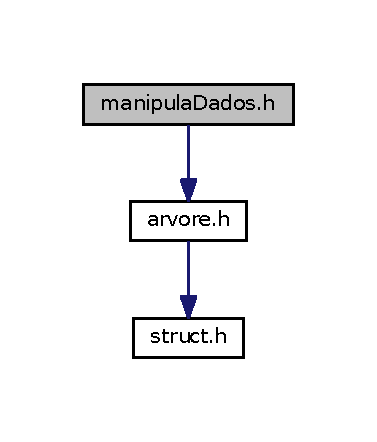
\includegraphics[width=181pt]{manipula_dados_8h__incl}
\end{center}
\end{figure}
Este grafo mostra quais são os ficheiros que incluem directamente ou indirectamente este ficheiro\+:\nopagebreak
\begin{figure}[H]
\begin{center}
\leavevmode
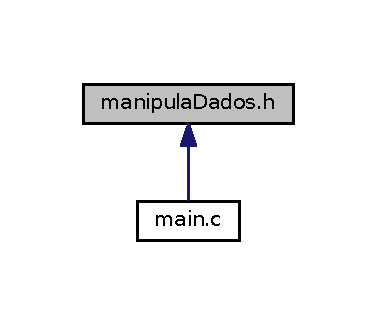
\includegraphics[width=181pt]{manipula_dados_8h__dep__incl}
\end{center}
\end{figure}
\subsection*{Funções}
\begin{DoxyCompactItemize}
\item 
\hyperlink{struct_8h_a1f5d65da7c19674431ada6dcf434b9ec}{Info} $\ast$ \hyperlink{manipula_dados_8h_ab97166de20d3d2dbd7ae675f067e6ded}{entrada\+Dados} (F\+I\+LE $\ast$entrada)
\begin{DoxyCompactList}\small\item\em Leitura dos dados do arquivo. \end{DoxyCompactList}\item 
int \hyperlink{manipula_dados_8h_a5668dd7fa2dce43515ae7f83015b18ef}{realiza\+Operacoes} (F\+I\+LE $\ast$operacoes, F\+I\+LE $\ast$saida, \hyperlink{struct_8h_a1f5d65da7c19674431ada6dcf434b9ec}{Info} $\ast$dados)
\begin{DoxyCompactList}\small\item\em Realização das operações nos dados recebidos. \end{DoxyCompactList}\end{DoxyCompactItemize}


\subsection{Descrição detalhada}
Arquivo que contém as principais funções do programa. 

\mbox{\Hypertarget{manipula_dados_8h_ab97166de20d3d2dbd7ae675f067e6ded}\label{manipula_dados_8h_ab97166de20d3d2dbd7ae675f067e6ded}} 
\index{manipula\+Dados.\+h@{manipula\+Dados.\+h}!entrada\+Dados@{entrada\+Dados}}
\index{entrada\+Dados@{entrada\+Dados}!manipula\+Dados.\+h@{manipula\+Dados.\+h}}
\subsubsection{\texorpdfstring{entrada\+Dados()}{entradaDados()}}
{\footnotesize\ttfamily \hyperlink{struct_8h_a1f5d65da7c19674431ada6dcf434b9ec}{Info}$\ast$ entrada\+Dados (\begin{DoxyParamCaption}\item[{F\+I\+LE $\ast$}]{entrada }\end{DoxyParamCaption})}



Leitura dos dados do arquivo. 

A função \hyperlink{manipula_dados_8h_ab97166de20d3d2dbd7ae675f067e6ded}{entrada\+Dados()} realiza a leitura dos dados do arquivo de entrada, manipulando as outras funções do programa, fazendo com que cada valor termine em sua devida estrutura, pronta para ser utilizada pela função \hyperlink{manipula_dados_8h_a5668dd7fa2dce43515ae7f83015b18ef}{realiza\+Operacoes()}.


\begin{DoxyParams}{Parâmetros}
{\em entrada} & Nome do arquivo de entrada\\
\hline
\end{DoxyParams}
\begin{DoxyReturn}{Retorna}
{\ttfamily Info$\ast$} contendo a árvore com as consultas e a lista de termos totais do arquivo. 
\end{DoxyReturn}
Grafo de chamadas desta função\+:\nopagebreak
\begin{figure}[H]
\begin{center}
\leavevmode
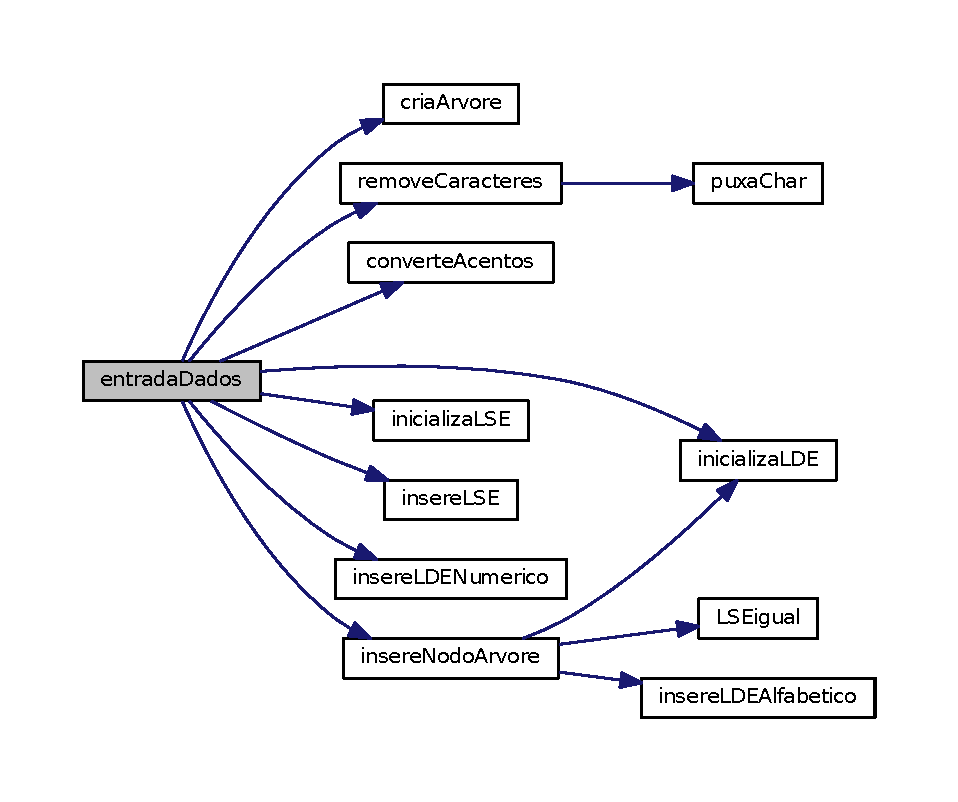
\includegraphics[width=350pt]{manipula_dados_8h_ab97166de20d3d2dbd7ae675f067e6ded_cgraph}
\end{center}
\end{figure}
\mbox{\Hypertarget{manipula_dados_8h_a5668dd7fa2dce43515ae7f83015b18ef}\label{manipula_dados_8h_a5668dd7fa2dce43515ae7f83015b18ef}} 
\index{manipula\+Dados.\+h@{manipula\+Dados.\+h}!realiza\+Operacoes@{realiza\+Operacoes}}
\index{realiza\+Operacoes@{realiza\+Operacoes}!manipula\+Dados.\+h@{manipula\+Dados.\+h}}
\subsubsection{\texorpdfstring{realiza\+Operacoes()}{realizaOperacoes()}}
{\footnotesize\ttfamily int realiza\+Operacoes (\begin{DoxyParamCaption}\item[{F\+I\+LE $\ast$}]{operacoes,  }\item[{F\+I\+LE $\ast$}]{saida,  }\item[{\hyperlink{struct_8h_a1f5d65da7c19674431ada6dcf434b9ec}{Info} $\ast$}]{dados }\end{DoxyParamCaption})}



Realização das operações nos dados recebidos. 

A função \hyperlink{manipula_dados_8h_a5668dd7fa2dce43515ae7f83015b18ef}{realiza\+Operacoes()} realiza a leitura das operacoes, realizando buscas nos dados fazendo com que toda a informação solicitada seja escrita no arquivo de saída.


\begin{DoxyParams}{Parâmetros}
{\em operacoes} & Nome do arquivo que contém as operações a serem realizadas nos {\ttfamily dados}. \\
\hline
{\em saida} & Nome do arquivo no qual serão escritos os dados de saída \\
\hline
{\em dados} & Informações geradas pela função \hyperlink{manipula_dados_8h_ab97166de20d3d2dbd7ae675f067e6ded}{entrada\+Dados()} a partir dos dados que haviam no arquivo de entrada. \\
\hline
\end{DoxyParams}
\begin{DoxyReturn}{Retorna}
{\ttfamily int} que representa a quantidade de operações realizadas. 
\end{DoxyReturn}

\hypertarget{manipula_string_8h}{}\section{Referência ao ficheiro manipula\+String.\+h}
\label{manipula_string_8h}\index{manipula\+String.\+h@{manipula\+String.\+h}}


Arquivo que contém funções relacionadas a manipulação de strings.  


Este grafo mostra quais são os ficheiros que incluem directamente ou indirectamente este ficheiro\+:\nopagebreak
\begin{figure}[H]
\begin{center}
\leavevmode
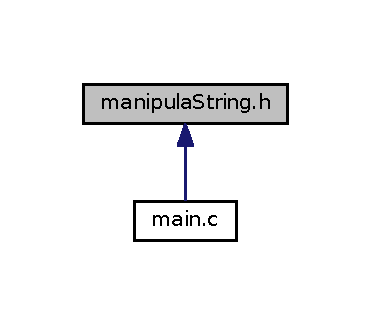
\includegraphics[width=178pt]{manipula_string_8h__dep__incl}
\end{center}
\end{figure}
\subsection*{Funções}
\begin{DoxyCompactItemize}
\item 
void \hyperlink{manipula_string_8h_a63ed716824573bfcd51287ae437ff9dc}{converte\+Acentos} (char $\ast$str)
\begin{DoxyCompactList}\small\item\em Tira os acentos de uma string. \end{DoxyCompactList}\item 
void \hyperlink{manipula_string_8h_a70ab0b22606dc0c70c1fc42a17c2dff0}{remove\+Caracteres} (char $\ast$str)
\begin{DoxyCompactList}\small\item\em Remove não-\/letras de uma string. \end{DoxyCompactList}\item 
void \hyperlink{manipula_string_8h_a20a57ce9614b104d137a3c3037f4f574}{puxa\+Char} (char $\ast$c)
\begin{DoxyCompactList}\small\item\em Remove um caractere de uma string. \end{DoxyCompactList}\end{DoxyCompactItemize}


\subsection{Descrição detalhada}
Arquivo que contém funções relacionadas a manipulação de strings. 

\mbox{\Hypertarget{manipula_string_8h_a63ed716824573bfcd51287ae437ff9dc}\label{manipula_string_8h_a63ed716824573bfcd51287ae437ff9dc}} 
\index{manipula\+String.\+h@{manipula\+String.\+h}!converte\+Acentos@{converte\+Acentos}}
\index{converte\+Acentos@{converte\+Acentos}!manipula\+String.\+h@{manipula\+String.\+h}}
\subsubsection{\texorpdfstring{converte\+Acentos()}{converteAcentos()}}
{\footnotesize\ttfamily void converte\+Acentos (\begin{DoxyParamCaption}\item[{char $\ast$}]{str }\end{DoxyParamCaption})}



Tira os acentos de uma string. 

A função \hyperlink{manipula_string_8h_a63ed716824573bfcd51287ae437ff9dc}{converte\+Acentos()} tira todos os acentos de uma string, transformando, i.\+e. à -\/$>$ a 
\begin{DoxyParams}{Parâmetros}
{\em str} & String que será convertida\\
\hline
\end{DoxyParams}
\begin{DoxyWarning}{Aviso}
A função funciona com strings escritas dentro do terminal, porém se for lido de um arquivo, pode ser que não funcione por causa das diferentes codificações. 
\end{DoxyWarning}
Este é o diagrama das funções que utilizam esta função\+:\nopagebreak
\begin{figure}[H]
\begin{center}
\leavevmode
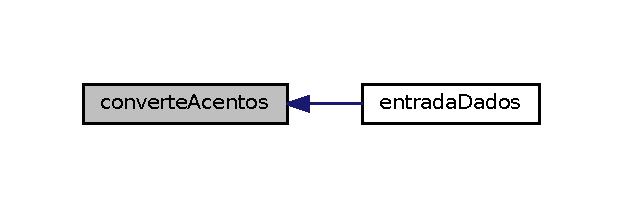
\includegraphics[width=299pt]{manipula_string_8h_a63ed716824573bfcd51287ae437ff9dc_icgraph}
\end{center}
\end{figure}
\mbox{\Hypertarget{manipula_string_8h_a20a57ce9614b104d137a3c3037f4f574}\label{manipula_string_8h_a20a57ce9614b104d137a3c3037f4f574}} 
\index{manipula\+String.\+h@{manipula\+String.\+h}!puxa\+Char@{puxa\+Char}}
\index{puxa\+Char@{puxa\+Char}!manipula\+String.\+h@{manipula\+String.\+h}}
\subsubsection{\texorpdfstring{puxa\+Char()}{puxaChar()}}
{\footnotesize\ttfamily void puxa\+Char (\begin{DoxyParamCaption}\item[{char $\ast$}]{c }\end{DoxyParamCaption})}



Remove um caractere de uma string. 

A função \hyperlink{manipula_string_8h_a20a57ce9614b104d137a3c3037f4f574}{puxa\+Char()} é a função auxiliar da \hyperlink{manipula_string_8h_a70ab0b22606dc0c70c1fc42a17c2dff0}{remove\+Caracteres()}. Ela remove um caractere de uma string, \char`\"{}puxando\char`\"{} todos os outros caracteres para não ficar um buraco no lugar do caractere a ser removido. 
\begin{DoxyParams}{Parâmetros}
{\em c} & Caractere a ser removido.\\
\hline
\end{DoxyParams}
\begin{DoxyNote}{Nota}
A função precisa que esse caractere esteja dentro de uma string, já que puxará todos os caracteres até encontrar um \textquotesingle{}\textbackslash{}0\textquotesingle{}. 
\end{DoxyNote}
Este é o diagrama das funções que utilizam esta função\+:\nopagebreak
\begin{figure}[H]
\begin{center}
\leavevmode
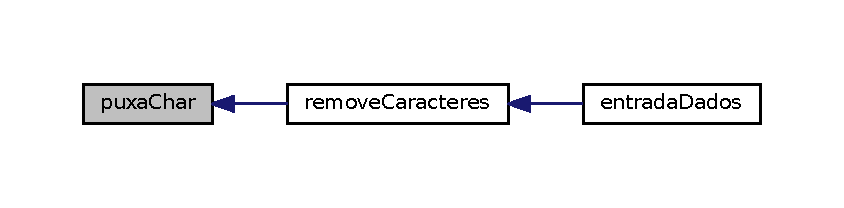
\includegraphics[width=350pt]{manipula_string_8h_a20a57ce9614b104d137a3c3037f4f574_icgraph}
\end{center}
\end{figure}
\mbox{\Hypertarget{manipula_string_8h_a70ab0b22606dc0c70c1fc42a17c2dff0}\label{manipula_string_8h_a70ab0b22606dc0c70c1fc42a17c2dff0}} 
\index{manipula\+String.\+h@{manipula\+String.\+h}!remove\+Caracteres@{remove\+Caracteres}}
\index{remove\+Caracteres@{remove\+Caracteres}!manipula\+String.\+h@{manipula\+String.\+h}}
\subsubsection{\texorpdfstring{remove\+Caracteres()}{removeCaracteres()}}
{\footnotesize\ttfamily void remove\+Caracteres (\begin{DoxyParamCaption}\item[{char $\ast$}]{str }\end{DoxyParamCaption})}



Remove não-\/letras de uma string. 

A função \hyperlink{manipula_string_8h_a70ab0b22606dc0c70c1fc42a17c2dff0}{remove\+Caracteres()} tira todos os caracteres que não sejam letras e/ou números de uma string. 
\begin{DoxyParams}{Parâmetros}
{\em str} & String na qual será feita a remoção \\
\hline
\end{DoxyParams}
Grafo de chamadas desta função\+:\nopagebreak
\begin{figure}[H]
\begin{center}
\leavevmode
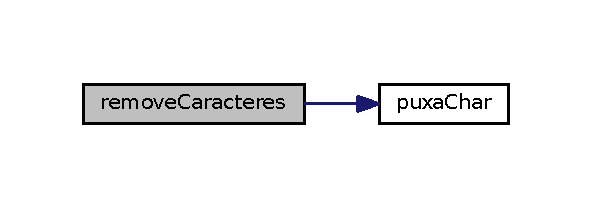
\includegraphics[width=284pt]{manipula_string_8h_a70ab0b22606dc0c70c1fc42a17c2dff0_cgraph}
\end{center}
\end{figure}
Este é o diagrama das funções que utilizam esta função\+:\nopagebreak
\begin{figure}[H]
\begin{center}
\leavevmode
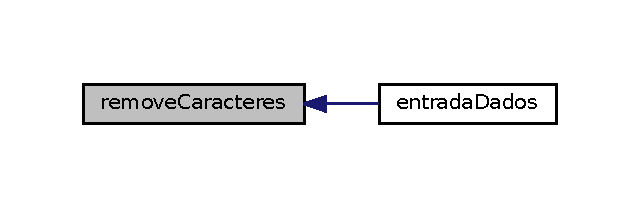
\includegraphics[width=307pt]{manipula_string_8h_a70ab0b22606dc0c70c1fc42a17c2dff0_icgraph}
\end{center}
\end{figure}

\hypertarget{operacoes_8h}{}\section{Referência ao ficheiro operacoes.\+h}
\label{operacoes_8h}\index{operacoes.\+h@{operacoes.\+h}}


Arquivo que contém funções executadas durante a leitura do arquivo de operacoes.  


{\ttfamily \#include \char`\"{}struct.\+h\char`\"{}}\newline
Diagrama de dependências de inclusão para operacoes.\+h\+:\nopagebreak
\begin{figure}[H]
\begin{center}
\leavevmode
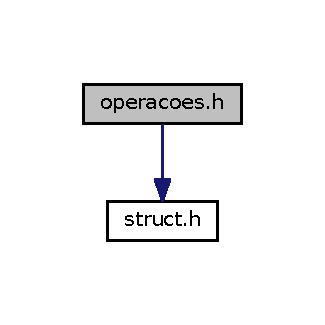
\includegraphics[width=156pt]{operacoes_8h__incl}
\end{center}
\end{figure}
\subsection*{Macros}
\begin{DoxyCompactItemize}
\item 
\mbox{\Hypertarget{operacoes_8h_a225c23d35d36fa87cd1a055c47d5b00b}\label{operacoes_8h_a225c23d35d36fa87cd1a055c47d5b00b}} 
\#define {\bfseries T\+A\+M\+\_\+\+V\+ET}~11000
\end{DoxyCompactItemize}
\subsection*{Funções}
\begin{DoxyCompactItemize}
\item 
void \hyperlink{operacoes_8h_a51685935591ec37d31c3a5600fe3f721}{consultas\+Por\+Localidade} (\hyperlink{struct_8h_a1664119ce88635d3bf4655a988ef8248}{Consulta} $\ast$arvore, char $\ast$cidade, int qtd\+Consultas, F\+I\+LE $\ast$saida)
\begin{DoxyCompactList}\small\item\em Encontra e escreve em um arquivo as consultas mais realizadas em uma dada cidade. \end{DoxyCompactList}\item 
int \hyperlink{operacoes_8h_a561e45bc2d18732cb0d4d8ebc678b82a}{consultas\+Arquivo} (\hyperlink{struct_8h_a1664119ce88635d3bf4655a988ef8248}{Consulta} $\ast$arvore, \hyperlink{struct_8h_a1664119ce88635d3bf4655a988ef8248}{Consulta} retorno\mbox{[}$\,$\mbox{]}, int qtd\+Consultas)
\begin{DoxyCompactList}\small\item\em Encontra as consultas mais realizadas em todo o arquivo. \end{DoxyCompactList}\item 
\hyperlink{struct_8h_ae030205799002e4fc414e374283d8598}{L\+DE} $\ast$ \hyperlink{operacoes_8h_a8375d33a9e2f1d5a7fa40eadbfd59ad3}{termos\+Por\+Localidade} (\hyperlink{struct_8h_a1664119ce88635d3bf4655a988ef8248}{Consulta} $\ast$arvore, \hyperlink{struct_8h_ae030205799002e4fc414e374283d8598}{L\+DE} $\ast$lista, char cidade\mbox{[}$\,$\mbox{]})
\begin{DoxyCompactList}\small\item\em Encontra os termos consultados em uma localidade. \end{DoxyCompactList}\item 
\hyperlink{struct_8h_ae030205799002e4fc414e374283d8598}{L\+DE} $\ast$ \hyperlink{operacoes_8h_ac04e2f9df7f7b0f31c80a7aa7f76297d}{termos\+Arquivo} (\hyperlink{struct_8h_ae030205799002e4fc414e374283d8598}{L\+DE} $\ast$lista\+Termos)
\begin{DoxyCompactList}\small\item\em Encontra os termos consultados em um arquivo. \end{DoxyCompactList}\item 
int \hyperlink{operacoes_8h_a0a89b388688c0c63b01d94d527c3ec88}{media\+Tamanho\+Consultas\+Localidade} (\hyperlink{struct_8h_a1664119ce88635d3bf4655a988ef8248}{Consulta} $\ast$arvore, char $\ast$cidade)
\begin{DoxyCompactList}\small\item\em Retorna a média do tamanho das consultas realizadas em uma cidade. \end{DoxyCompactList}\item 
int \hyperlink{operacoes_8h_abfc720731dce4781dfd389ee245f3821}{media\+Tamanho\+Consultas\+Arquivo} (\hyperlink{struct_8h_a1664119ce88635d3bf4655a988ef8248}{Consulta} $\ast$arvore)
\begin{DoxyCompactList}\small\item\em Retorna a média do tamanho das consultas realizadas em todo o arquivo. \end{DoxyCompactList}\item 
\hyperlink{struct_8h_ae030205799002e4fc414e374283d8598}{L\+DE} $\ast$ \hyperlink{operacoes_8h_a4fe0890a6b92b76e2651aed7326988ad}{insere\+Termos\+Nodo} (\hyperlink{struct_8h_ae030205799002e4fc414e374283d8598}{L\+DE} $\ast$lista, \hyperlink{struct_8h_a0d3de75d86bf1db6f749c91f755b870c}{L\+SE} $\ast$termos, int qtde)
\begin{DoxyCompactList}\small\item\em Concatena todos os termos de uma L\+SE em uma L\+DE. \end{DoxyCompactList}\item 
void \hyperlink{operacoes_8h_ad5c8115288084f240afe157a2d62c433}{auxiliar\+Media\+Tamanho\+Consultas\+Arquivo} (\hyperlink{struct_8h_a1664119ce88635d3bf4655a988ef8248}{Consulta} $\ast$arvore, int $\ast$tot\+Termos, int $\ast$tot\+Consultas)
\begin{DoxyCompactList}\small\item\em Calcula a quantidade total de consultas e a quantidade total de termos no arquivo. \end{DoxyCompactList}\item 
void \hyperlink{operacoes_8h_a00195a3339794084b2ceb879da73642e}{auxiliar\+Media\+Tamanho\+Consultas\+Localidade} (\hyperlink{struct_8h_a1664119ce88635d3bf4655a988ef8248}{Consulta} $\ast$arvore, int $\ast$tot\+Termos, int $\ast$tot\+Consultas, char $\ast$cidade)
\begin{DoxyCompactList}\small\item\em Calcula a quantidade total de consultas e a quantidade total de termos em uma dada cidade. \end{DoxyCompactList}\item 
int \hyperlink{operacoes_8h_a3af226df14ca18acf9c3de7d605004d5}{tem\+Cidade\+Na\+Lista} (char $\ast$cidade, \hyperlink{struct_8h_ae030205799002e4fc414e374283d8598}{L\+DE} $\ast$lista)
\begin{DoxyCompactList}\small\item\em Retorna a \char`\"{}quantidade\char`\"{} de vezes que um termo aparece em uma L\+DE. \end{DoxyCompactList}\item 
int \hyperlink{operacoes_8h_a8679d0e9fceefc34588b098a6f3e235a}{acha\+Vetor\+Reps} (\hyperlink{struct_8h_a1664119ce88635d3bf4655a988ef8248}{Consulta} $\ast$arvore, int $\ast$vetor, int contador)
\begin{DoxyCompactList}\small\item\em Copia a quantidade de acessos de cada nodo da arvore pra posições de um vetor. \end{DoxyCompactList}\item 
int \hyperlink{operacoes_8h_a31658a0ce4d50f633b73cc410753ed58}{acha\+Vetor\+Reps\+Localidade} (\hyperlink{struct_8h_a1664119ce88635d3bf4655a988ef8248}{Consulta} $\ast$arvore, int $\ast$vetor, int contador, char $\ast$cidade, \hyperlink{struct_8h_a30e93d002c23d05f5d039449d6775eb6}{Qtdcons} $\ast$qtd\+Cons)
\begin{DoxyCompactList}\small\item\em Encontra as repetições de uma consulta por localidade. \end{DoxyCompactList}\item 
int \hyperlink{operacoes_8h_a670217d6418d7f242b8529dc3a07eefa}{copia\+Arvore} (\hyperlink{struct_8h_a1664119ce88635d3bf4655a988ef8248}{Consulta} $\ast$arvore, \hyperlink{struct_8h_a1664119ce88635d3bf4655a988ef8248}{Consulta} $\ast$retorno, int $\ast$vetor, int qtd, int pos, int vezes\+Rep)
\begin{DoxyCompactList}\small\item\em Copia uma arvore para a outra, de maneira ordenada. \end{DoxyCompactList}\item 
void \hyperlink{operacoes_8h_aabe9eba415b4b21ad403b5dff86c83a4}{quick\+\_\+sort} (int $\ast$a, int left, int right)
\begin{DoxyCompactList}\small\item\em Quick sort de vetores int genéricos. \end{DoxyCompactList}\end{DoxyCompactItemize}


\subsection{Descrição detalhada}
Arquivo que contém funções executadas durante a leitura do arquivo de operacoes. 

\mbox{\Hypertarget{operacoes_8h_a8679d0e9fceefc34588b098a6f3e235a}\label{operacoes_8h_a8679d0e9fceefc34588b098a6f3e235a}} 
\index{operacoes.\+h@{operacoes.\+h}!acha\+Vetor\+Reps@{acha\+Vetor\+Reps}}
\index{acha\+Vetor\+Reps@{acha\+Vetor\+Reps}!operacoes.\+h@{operacoes.\+h}}
\subsubsection{\texorpdfstring{acha\+Vetor\+Reps()}{achaVetorReps()}}
{\footnotesize\ttfamily int acha\+Vetor\+Reps (\begin{DoxyParamCaption}\item[{\hyperlink{struct_8h_a1664119ce88635d3bf4655a988ef8248}{Consulta} $\ast$}]{arvore,  }\item[{int $\ast$}]{vetor,  }\item[{int}]{contador }\end{DoxyParamCaption})}



Copia a quantidade de acessos de cada nodo da arvore pra posições de um vetor. 

A função \hyperlink{operacoes_8h_a8679d0e9fceefc34588b098a6f3e235a}{acha\+Vetor\+Reps()} recebe uma arvore, e pra cada nodo dessa árvore encontrado recursivamente, copia a quantidade de acessos dele para um vetor


\begin{DoxyParams}{Parâmetros}
{\em arvore} & Arvore que contem as informações a serem inseridas em vetor \\
\hline
{\em vetor} & Vetor com as quantidades de consultas realizadas. \\
\hline
{\em contador} & Conta em qual posição de {\ttfamily vetor} será inserido a quantidade \\
\hline
\end{DoxyParams}
\begin{DoxyReturn}{Retorna}
{\ttfamily int} Quantidade de consultas encontradas 
\end{DoxyReturn}
\begin{DoxyNote}{Nota}
Essa função é uma função auxiliar para \hyperlink{operacoes_8h_a561e45bc2d18732cb0d4d8ebc678b82a}{consultas\+Arquivo()} 
\end{DoxyNote}
\mbox{\Hypertarget{operacoes_8h_a31658a0ce4d50f633b73cc410753ed58}\label{operacoes_8h_a31658a0ce4d50f633b73cc410753ed58}} 
\index{operacoes.\+h@{operacoes.\+h}!acha\+Vetor\+Reps\+Localidade@{acha\+Vetor\+Reps\+Localidade}}
\index{acha\+Vetor\+Reps\+Localidade@{acha\+Vetor\+Reps\+Localidade}!operacoes.\+h@{operacoes.\+h}}
\subsubsection{\texorpdfstring{acha\+Vetor\+Reps\+Localidade()}{achaVetorRepsLocalidade()}}
{\footnotesize\ttfamily int acha\+Vetor\+Reps\+Localidade (\begin{DoxyParamCaption}\item[{\hyperlink{struct_8h_a1664119ce88635d3bf4655a988ef8248}{Consulta} $\ast$}]{arvore,  }\item[{int $\ast$}]{vetor,  }\item[{int}]{contador,  }\item[{char $\ast$}]{cidade,  }\item[{\hyperlink{struct_8h_a30e93d002c23d05f5d039449d6775eb6}{Qtdcons} $\ast$}]{qtd\+Cons }\end{DoxyParamCaption})}



Encontra as repetições de uma consulta por localidade. 

A função \hyperlink{operacoes_8h_a31658a0ce4d50f633b73cc410753ed58}{acha\+Vetor\+Reps\+Localidade()} recebe uma estrutura especial, criada somente para ela, fazendo com que ela coloque em um vetor, todas as consultas realizadas em uma cidade.


\begin{DoxyParams}{Parâmetros}
{\em arvore} & Arvore que contem as informações a serem inseridas em vetor \\
\hline
{\em vetor} & Vetor com as quantidades de consultas realizadas. \\
\hline
{\em contador} & Conta em qual posição de {\ttfamily vetor} será inserido a quantidade \\
\hline
{\em cidade} & Cidade a qual estamos procurando as consultas \\
\hline
{\em qtd\+Cons} & Vetor de Qtd\+Cons onde serão guardados as consultas e sua quantidade \\
\hline
\end{DoxyParams}
\begin{DoxyReturn}{Retorna}
{\ttfamily int} Quantidade de consultas encontradas 
\end{DoxyReturn}
\begin{DoxyNote}{Nota}
Essa função é uma função auxiliar para \hyperlink{operacoes_8h_a51685935591ec37d31c3a5600fe3f721}{consultas\+Por\+Localidade()} 
\end{DoxyNote}
Grafo de chamadas desta função\+:\nopagebreak
\begin{figure}[H]
\begin{center}
\leavevmode
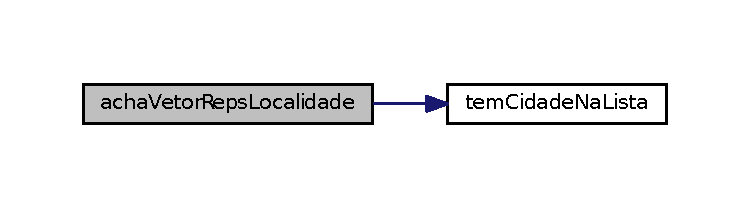
\includegraphics[width=350pt]{operacoes_8h_a31658a0ce4d50f633b73cc410753ed58_cgraph}
\end{center}
\end{figure}
\mbox{\Hypertarget{operacoes_8h_ad5c8115288084f240afe157a2d62c433}\label{operacoes_8h_ad5c8115288084f240afe157a2d62c433}} 
\index{operacoes.\+h@{operacoes.\+h}!auxiliar\+Media\+Tamanho\+Consultas\+Arquivo@{auxiliar\+Media\+Tamanho\+Consultas\+Arquivo}}
\index{auxiliar\+Media\+Tamanho\+Consultas\+Arquivo@{auxiliar\+Media\+Tamanho\+Consultas\+Arquivo}!operacoes.\+h@{operacoes.\+h}}
\subsubsection{\texorpdfstring{auxiliar\+Media\+Tamanho\+Consultas\+Arquivo()}{auxiliarMediaTamanhoConsultasArquivo()}}
{\footnotesize\ttfamily void auxiliar\+Media\+Tamanho\+Consultas\+Arquivo (\begin{DoxyParamCaption}\item[{\hyperlink{struct_8h_a1664119ce88635d3bf4655a988ef8248}{Consulta} $\ast$}]{arvore,  }\item[{int $\ast$}]{tot\+Termos,  }\item[{int $\ast$}]{tot\+Consultas }\end{DoxyParamCaption})}



Calcula a quantidade total de consultas e a quantidade total de termos no arquivo. 

A função \hyperlink{operacoes_8h_ad5c8115288084f240afe157a2d62c433}{auxiliar\+Media\+Tamanho\+Consultas\+Arquivo()} varre uma arvore buscando a quantidade total de consultas assim como a quantidade total de termos que possuem naquela arvore.


\begin{DoxyParams}{Parâmetros}
{\em arvore} & Arvore a ser varrida \\
\hline
{\em tot\+Termos} & Ponteiro para um inteiro que armazena a quantidade total de termos na árvore \\
\hline
{\em tot\+Consultas} & Ponteiro para um inteiro que armazena a quantidade total de consultas na árvore \\
\hline
\end{DoxyParams}
\begin{DoxyNote}{Nota}
Essa função é uma função auxiliar para \hyperlink{operacoes_8h_abfc720731dce4781dfd389ee245f3821}{media\+Tamanho\+Consultas\+Arquivo()} 
\end{DoxyNote}
Este é o diagrama das funções que utilizam esta função\+:\nopagebreak
\begin{figure}[H]
\begin{center}
\leavevmode

\includegraphics[width=350pt]{operacoes_8h_ad5c8115288084f240afe157a2d62c433_icgraph}
\end{center}
\end{figure}
\mbox{\Hypertarget{operacoes_8h_a00195a3339794084b2ceb879da73642e}\label{operacoes_8h_a00195a3339794084b2ceb879da73642e}} 
\index{operacoes.\+h@{operacoes.\+h}!auxiliar\+Media\+Tamanho\+Consultas\+Localidade@{auxiliar\+Media\+Tamanho\+Consultas\+Localidade}}
\index{auxiliar\+Media\+Tamanho\+Consultas\+Localidade@{auxiliar\+Media\+Tamanho\+Consultas\+Localidade}!operacoes.\+h@{operacoes.\+h}}
\subsubsection{\texorpdfstring{auxiliar\+Media\+Tamanho\+Consultas\+Localidade()}{auxiliarMediaTamanhoConsultasLocalidade()}}
{\footnotesize\ttfamily void auxiliar\+Media\+Tamanho\+Consultas\+Localidade (\begin{DoxyParamCaption}\item[{\hyperlink{struct_8h_a1664119ce88635d3bf4655a988ef8248}{Consulta} $\ast$}]{arvore,  }\item[{int $\ast$}]{tot\+Termos,  }\item[{int $\ast$}]{tot\+Consultas,  }\item[{char $\ast$}]{cidade }\end{DoxyParamCaption})}



Calcula a quantidade total de consultas e a quantidade total de termos em uma dada cidade. 

A função \hyperlink{operacoes_8h_a00195a3339794084b2ceb879da73642e}{auxiliar\+Media\+Tamanho\+Consultas\+Localidade()} varre uma arvore buscando a quantidade total de consultas assim como a quantidade total de termos que possuem naquela arvore e que tenham acontecido nas consultas de uma determinada cidade


\begin{DoxyParams}{Parâmetros}
{\em arvore} & Arvore a ser varrida \\
\hline
{\em tot\+Termos} & Ponteiro para um inteiro que armazena a quantidade total de termos consultados pela cidade na árvore \\
\hline
{\em tot\+Consultas} & Ponteiro para um inteiro que armazena a quantidade total de consultas realizadas pela cidade na árvore \\
\hline
{\em cidade} & String com o nome da cidade que está sendo procurada \\
\hline
\end{DoxyParams}
\begin{DoxyNote}{Nota}
Essa função é uma função auxiliar para \hyperlink{operacoes_8h_a0a89b388688c0c63b01d94d527c3ec88}{media\+Tamanho\+Consultas\+Localidade()} 
\end{DoxyNote}
Grafo de chamadas desta função\+:\nopagebreak
\begin{figure}[H]
\begin{center}
\leavevmode

\includegraphics[width=350pt]{operacoes_8h_a00195a3339794084b2ceb879da73642e_cgraph}
\end{center}
\end{figure}
Este é o diagrama das funções que utilizam esta função\+:\nopagebreak
\begin{figure}[H]
\begin{center}
\leavevmode
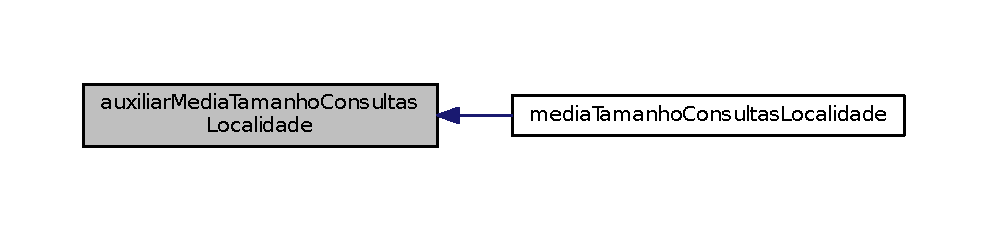
\includegraphics[width=350pt]{operacoes_8h_a00195a3339794084b2ceb879da73642e_icgraph}
\end{center}
\end{figure}
\mbox{\Hypertarget{operacoes_8h_a561e45bc2d18732cb0d4d8ebc678b82a}\label{operacoes_8h_a561e45bc2d18732cb0d4d8ebc678b82a}} 
\index{operacoes.\+h@{operacoes.\+h}!consultas\+Arquivo@{consultas\+Arquivo}}
\index{consultas\+Arquivo@{consultas\+Arquivo}!operacoes.\+h@{operacoes.\+h}}
\subsubsection{\texorpdfstring{consultas\+Arquivo()}{consultasArquivo()}}
{\footnotesize\ttfamily int consultas\+Arquivo (\begin{DoxyParamCaption}\item[{\hyperlink{struct_8h_a1664119ce88635d3bf4655a988ef8248}{Consulta} $\ast$}]{arvore,  }\item[{\hyperlink{struct_8h_a1664119ce88635d3bf4655a988ef8248}{Consulta}}]{retorno\mbox{[}$\,$\mbox{]},  }\item[{int}]{qtd\+Consultas }\end{DoxyParamCaption})}



Encontra as consultas mais realizadas em todo o arquivo. 

A função \hyperlink{operacoes_8h_a561e45bc2d18732cb0d4d8ebc678b82a}{consultas\+Arquivo()} encontra as consultas que foram mais buscadas. Se 0 for passado como parametro para {\ttfamily qtd\+Consultas}, são mostradas todas as consultas realizadas.


\begin{DoxyParams}{Parâmetros}
{\em arvore} & Arvore que contem os dados \\
\hline
{\em retorno} & Array de tamanho {\ttfamily qtd\+Consultas} (inicialmente), contendo as {\ttfamily qtd\+Consultas} mais realizadas em todo o arquivo \\
\hline
{\em qtd\+Consultas} & Quantidade de consultas que serão buscadas na {\ttfamily arvore}.\\
\hline
\end{DoxyParams}
\begin{DoxyReturn}{Retorna}
{\ttfamily int} que é a quantidade de elementos em {\ttfamily retorno}. 
\end{DoxyReturn}
\begin{DoxyWarning}{Aviso}
Essa função é extremamente custosa quando se está procurando T\+O\+D\+AS as consultas do arquivo. 
\end{DoxyWarning}
\mbox{\Hypertarget{operacoes_8h_a51685935591ec37d31c3a5600fe3f721}\label{operacoes_8h_a51685935591ec37d31c3a5600fe3f721}} 
\index{operacoes.\+h@{operacoes.\+h}!consultas\+Por\+Localidade@{consultas\+Por\+Localidade}}
\index{consultas\+Por\+Localidade@{consultas\+Por\+Localidade}!operacoes.\+h@{operacoes.\+h}}
\subsubsection{\texorpdfstring{consultas\+Por\+Localidade()}{consultasPorLocalidade()}}
{\footnotesize\ttfamily void consultas\+Por\+Localidade (\begin{DoxyParamCaption}\item[{\hyperlink{struct_8h_a1664119ce88635d3bf4655a988ef8248}{Consulta} $\ast$}]{arvore,  }\item[{char $\ast$}]{cidade,  }\item[{int}]{qtd\+Consultas,  }\item[{F\+I\+LE $\ast$}]{saida }\end{DoxyParamCaption})}



Encontra e escreve em um arquivo as consultas mais realizadas em uma dada cidade. 

A função \hyperlink{operacoes_8h_a51685935591ec37d31c3a5600fe3f721}{consultas\+Por\+Localidade()} encontra e escreve em um arquivo as {\ttfamily qtd\+Consultas} mais realizadas em uma dada cidade. Se 0 for passado como parametro para {\ttfamily qtd\+Consultas}, são mostradas todas as consultas realizadas naquela localidade.


\begin{DoxyParams}{Parâmetros}
{\em arvore} & Arvore que contem os dados \\
\hline
{\em cidade} & String da cidade que estamos procurando os dados \\
\hline
{\em qtd\+Consultas} & Quantidade de consultas que serão printadas no arquivo \\
\hline
{\em saida} & Arquivo no qual serão printadas as {\ttfamily qtd\+Consultas} mais consultadas. \\
\hline
\end{DoxyParams}
\mbox{\Hypertarget{operacoes_8h_a670217d6418d7f242b8529dc3a07eefa}\label{operacoes_8h_a670217d6418d7f242b8529dc3a07eefa}} 
\index{operacoes.\+h@{operacoes.\+h}!copia\+Arvore@{copia\+Arvore}}
\index{copia\+Arvore@{copia\+Arvore}!operacoes.\+h@{operacoes.\+h}}
\subsubsection{\texorpdfstring{copia\+Arvore()}{copiaArvore()}}
{\footnotesize\ttfamily int copia\+Arvore (\begin{DoxyParamCaption}\item[{\hyperlink{struct_8h_a1664119ce88635d3bf4655a988ef8248}{Consulta} $\ast$}]{arvore,  }\item[{\hyperlink{struct_8h_a1664119ce88635d3bf4655a988ef8248}{Consulta} $\ast$}]{retorno,  }\item[{int $\ast$}]{vetor,  }\item[{int}]{qtd,  }\item[{int}]{pos,  }\item[{int}]{vezes\+Rep }\end{DoxyParamCaption})}



Copia uma arvore para a outra, de maneira ordenada. 

A função \hyperlink{operacoes_8h_a670217d6418d7f242b8529dc3a07eefa}{copia\+Arvore()} copia a arvore {\ttfamily arvore}, para a arvore {\ttfamily retorno}, de maneira ordenada, seguindo o ordenamento dado por {\ttfamily vetor} 


\begin{DoxyParams}{Parâmetros}
{\em arvore} & Arvore que contem as informações \\
\hline
{\em retorno} & Arvore para a qual serao copiados os valores \\
\hline
{\em vetor} & Vetor ordenado, com o qual procuramos os nodos certos a serem inseridos \\
\hline
{\em qtd} & Até qual posição de {\ttfamily vetor} preciso preencher \\
\hline
{\em pos} & Minha posição de preenchimento atual de {\ttfamily vetor} \\
\hline
{\em vezes\+Rep} & Vezes que a repetição ocorreu \\
\hline
\end{DoxyParams}
\begin{DoxyReturn}{Retorna}
{\ttfamily int} Usado dentro das recursões para saber em que repetição da recursão estamos 
\end{DoxyReturn}
\begin{DoxyNote}{Nota}
Essa função é uma função auxiliar para \hyperlink{operacoes_8h_a561e45bc2d18732cb0d4d8ebc678b82a}{consultas\+Arquivo()} 
\end{DoxyNote}
\mbox{\Hypertarget{operacoes_8h_a4fe0890a6b92b76e2651aed7326988ad}\label{operacoes_8h_a4fe0890a6b92b76e2651aed7326988ad}} 
\index{operacoes.\+h@{operacoes.\+h}!insere\+Termos\+Nodo@{insere\+Termos\+Nodo}}
\index{insere\+Termos\+Nodo@{insere\+Termos\+Nodo}!operacoes.\+h@{operacoes.\+h}}
\subsubsection{\texorpdfstring{insere\+Termos\+Nodo()}{insereTermosNodo()}}
{\footnotesize\ttfamily \hyperlink{struct_8h_ae030205799002e4fc414e374283d8598}{L\+DE}$\ast$ insere\+Termos\+Nodo (\begin{DoxyParamCaption}\item[{\hyperlink{struct_8h_ae030205799002e4fc414e374283d8598}{L\+DE} $\ast$}]{lista,  }\item[{\hyperlink{struct_8h_a0d3de75d86bf1db6f749c91f755b870c}{L\+SE} $\ast$}]{termos,  }\item[{int}]{qtde }\end{DoxyParamCaption})}



Concatena todos os termos de uma L\+SE em uma L\+DE. 

A função \hyperlink{operacoes_8h_a4fe0890a6b92b76e2651aed7326988ad}{insere\+Termos\+Nodo()} concatena todos os termos que existem em {\ttfamily termos} em {\ttfamily lista}. É passado como parametro numérico da função \hyperlink{lde_8h_a695bd097eab9845e2eddd196523c58ac}{insere\+L\+D\+E\+Numerico()} o que é recebido no parametro {\ttfamily qtde}.


\begin{DoxyParams}{Parâmetros}
{\em lista} & Lista que receberá os termos \\
\hline
{\em termos} & Lista da qual são copiados os termos \\
\hline
{\em qtde} & Valor que será passado como parametro para a função \hyperlink{lde_8h_a695bd097eab9845e2eddd196523c58ac}{insere\+L\+D\+E\+Numerico()}. É a quantidade de vezes que cada termo aparecia originalmente. \\
\hline
\end{DoxyParams}
\begin{DoxyReturn}{Retorna}
{\ttfamily L\+D\+E$\ast$} que é a {\ttfamily lista} com a adição dos novos termos. 
\end{DoxyReturn}
\begin{DoxyNote}{Nota}
Essa função é uma função auxiliar para \hyperlink{operacoes_8h_a8375d33a9e2f1d5a7fa40eadbfd59ad3}{termos\+Por\+Localidade()} 
\end{DoxyNote}
Grafo de chamadas desta função\+:\nopagebreak
\begin{figure}[H]
\begin{center}
\leavevmode
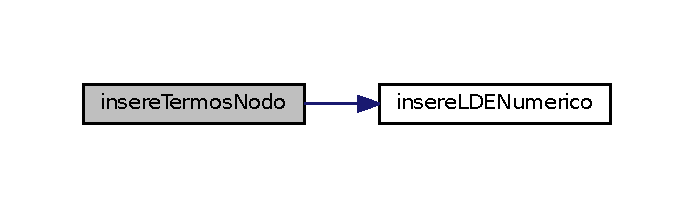
\includegraphics[width=333pt]{operacoes_8h_a4fe0890a6b92b76e2651aed7326988ad_cgraph}
\end{center}
\end{figure}
Este é o diagrama das funções que utilizam esta função\+:\nopagebreak
\begin{figure}[H]
\begin{center}
\leavevmode
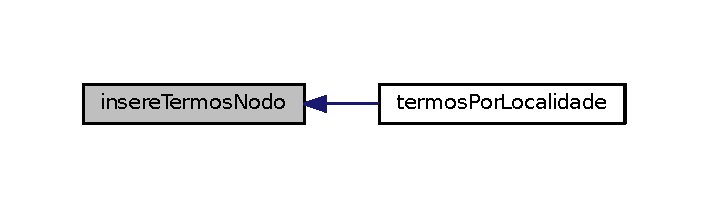
\includegraphics[width=340pt]{operacoes_8h_a4fe0890a6b92b76e2651aed7326988ad_icgraph}
\end{center}
\end{figure}
\mbox{\Hypertarget{operacoes_8h_abfc720731dce4781dfd389ee245f3821}\label{operacoes_8h_abfc720731dce4781dfd389ee245f3821}} 
\index{operacoes.\+h@{operacoes.\+h}!media\+Tamanho\+Consultas\+Arquivo@{media\+Tamanho\+Consultas\+Arquivo}}
\index{media\+Tamanho\+Consultas\+Arquivo@{media\+Tamanho\+Consultas\+Arquivo}!operacoes.\+h@{operacoes.\+h}}
\subsubsection{\texorpdfstring{media\+Tamanho\+Consultas\+Arquivo()}{mediaTamanhoConsultasArquivo()}}
{\footnotesize\ttfamily int media\+Tamanho\+Consultas\+Arquivo (\begin{DoxyParamCaption}\item[{\hyperlink{struct_8h_a1664119ce88635d3bf4655a988ef8248}{Consulta} $\ast$}]{arvore }\end{DoxyParamCaption})}



Retorna a média do tamanho das consultas realizadas em todo o arquivo. 

A função \hyperlink{operacoes_8h_abfc720731dce4781dfd389ee245f3821}{media\+Tamanho\+Consultas\+Arquivo()} retorna a média do tamanho das consultas realizadas em no arquivo 
\begin{DoxyParams}{Parâmetros}
{\em arvore} & Arvore com todas as consultas\\
\hline
\end{DoxyParams}
\begin{DoxyReturn}{Retorna}
{\ttfamily int$\ast$} que é a média do tamanho das consultas realizadas no arquivo 
\end{DoxyReturn}
Grafo de chamadas desta função\+:\nopagebreak
\begin{figure}[H]
\begin{center}
\leavevmode

\includegraphics[width=350pt]{operacoes_8h_abfc720731dce4781dfd389ee245f3821_cgraph}
\end{center}
\end{figure}
\mbox{\Hypertarget{operacoes_8h_a0a89b388688c0c63b01d94d527c3ec88}\label{operacoes_8h_a0a89b388688c0c63b01d94d527c3ec88}} 
\index{operacoes.\+h@{operacoes.\+h}!media\+Tamanho\+Consultas\+Localidade@{media\+Tamanho\+Consultas\+Localidade}}
\index{media\+Tamanho\+Consultas\+Localidade@{media\+Tamanho\+Consultas\+Localidade}!operacoes.\+h@{operacoes.\+h}}
\subsubsection{\texorpdfstring{media\+Tamanho\+Consultas\+Localidade()}{mediaTamanhoConsultasLocalidade()}}
{\footnotesize\ttfamily int media\+Tamanho\+Consultas\+Localidade (\begin{DoxyParamCaption}\item[{\hyperlink{struct_8h_a1664119ce88635d3bf4655a988ef8248}{Consulta} $\ast$}]{arvore,  }\item[{char $\ast$}]{cidade }\end{DoxyParamCaption})}



Retorna a média do tamanho das consultas realizadas em uma cidade. 

A função \hyperlink{operacoes_8h_a0a89b388688c0c63b01d94d527c3ec88}{media\+Tamanho\+Consultas\+Localidade()} retorna a média do tamanho das consultas realizadas em uma determinada localidade


\begin{DoxyParams}{Parâmetros}
{\em arvore} & Arvore com todas as consultas \\
\hline
{\em cidade} & Cidade a qual estamos procurando\\
\hline
\end{DoxyParams}
\begin{DoxyReturn}{Retorna}
{\ttfamily int$\ast$} que é a média do tamanho das consultas realizadas em uma determinada cidade. 
\end{DoxyReturn}
Grafo de chamadas desta função\+:\nopagebreak
\begin{figure}[H]
\begin{center}
\leavevmode

\includegraphics[width=350pt]{operacoes_8h_a0a89b388688c0c63b01d94d527c3ec88_cgraph}
\end{center}
\end{figure}
\mbox{\Hypertarget{operacoes_8h_aabe9eba415b4b21ad403b5dff86c83a4}\label{operacoes_8h_aabe9eba415b4b21ad403b5dff86c83a4}} 
\index{operacoes.\+h@{operacoes.\+h}!quick\+\_\+sort@{quick\+\_\+sort}}
\index{quick\+\_\+sort@{quick\+\_\+sort}!operacoes.\+h@{operacoes.\+h}}
\subsubsection{\texorpdfstring{quick\+\_\+sort()}{quick\_sort()}}
{\footnotesize\ttfamily void quick\+\_\+sort (\begin{DoxyParamCaption}\item[{int $\ast$}]{a,  }\item[{int}]{left,  }\item[{int}]{right }\end{DoxyParamCaption})}



Quick sort de vetores int genéricos. 

Ordena um vetor de int genéricos usando o algoritmo de Quick Sort (\href{https://pt.wikipedia.org/wiki/Quicksort}{\tt https\+://pt.\+wikipedia.\+org/wiki/\+Quicksort})


\begin{DoxyParams}{Parâmetros}
{\em a} & Vetor a ser ordenado \\
\hline
{\em left} & Detalhe de implementação relacionado ao algoritmo de Divide\&Conqueror \\
\hline
{\em right} & Detalhe de implementação relacionado ao algoritmo de Divide\&Conqueror \\
\hline
\end{DoxyParams}
\begin{DoxyNote}{Nota}
Essa função é uma função auxiliar 
\end{DoxyNote}
\mbox{\Hypertarget{operacoes_8h_a3af226df14ca18acf9c3de7d605004d5}\label{operacoes_8h_a3af226df14ca18acf9c3de7d605004d5}} 
\index{operacoes.\+h@{operacoes.\+h}!tem\+Cidade\+Na\+Lista@{tem\+Cidade\+Na\+Lista}}
\index{tem\+Cidade\+Na\+Lista@{tem\+Cidade\+Na\+Lista}!operacoes.\+h@{operacoes.\+h}}
\subsubsection{\texorpdfstring{tem\+Cidade\+Na\+Lista()}{temCidadeNaLista()}}
{\footnotesize\ttfamily int tem\+Cidade\+Na\+Lista (\begin{DoxyParamCaption}\item[{char $\ast$}]{cidade,  }\item[{\hyperlink{struct_8h_ae030205799002e4fc414e374283d8598}{L\+DE} $\ast$}]{lista }\end{DoxyParamCaption})}



Retorna a \char`\"{}quantidade\char`\"{} de vezes que um termo aparece em uma L\+DE. 

A função \hyperlink{operacoes_8h_a3af226df14ca18acf9c3de7d605004d5}{tem\+Cidade\+Na\+Lista()} varre uma L\+DE, procurando um termo identico a {\ttfamily cidade}. Caso exista esse termo na L\+DE, retorna a \char`\"{}quantidade\char`\"{} de vezes que ele ocorre, caso contrário retorna 0. Essa $<$quantidade de vezes que ele ocorre$>$ é dada pelo campo \hyperlink{structlde_aa8a45bf920d47706309cd931134d5219}{L\+D\+E\+::qtde} da cidade.


\begin{DoxyParams}{Parâmetros}
{\em cidade} & String a ser procurada em {\ttfamily lista} \\
\hline
{\em lista} & Lista que será varrida procurando por {\ttfamily cidade} \\
\hline
\end{DoxyParams}
\begin{DoxyReturn}{Retorna}
{\ttfamily int} 1 se existe a string na lista e 0 se não existe a string na lista 
\end{DoxyReturn}
\begin{DoxyNote}{Nota}
Essa função é uma função auxiliar para \hyperlink{operacoes_8h_a31658a0ce4d50f633b73cc410753ed58}{acha\+Vetor\+Reps\+Localidade()}, \hyperlink{operacoes_8h_a00195a3339794084b2ceb879da73642e}{auxiliar\+Media\+Tamanho\+Consultas\+Localidade()} e \hyperlink{operacoes_8h_a8375d33a9e2f1d5a7fa40eadbfd59ad3}{termos\+Por\+Localidade()} 
\end{DoxyNote}
Este é o diagrama das funções que utilizam esta função\+:\nopagebreak
\begin{figure}[H]
\begin{center}
\leavevmode
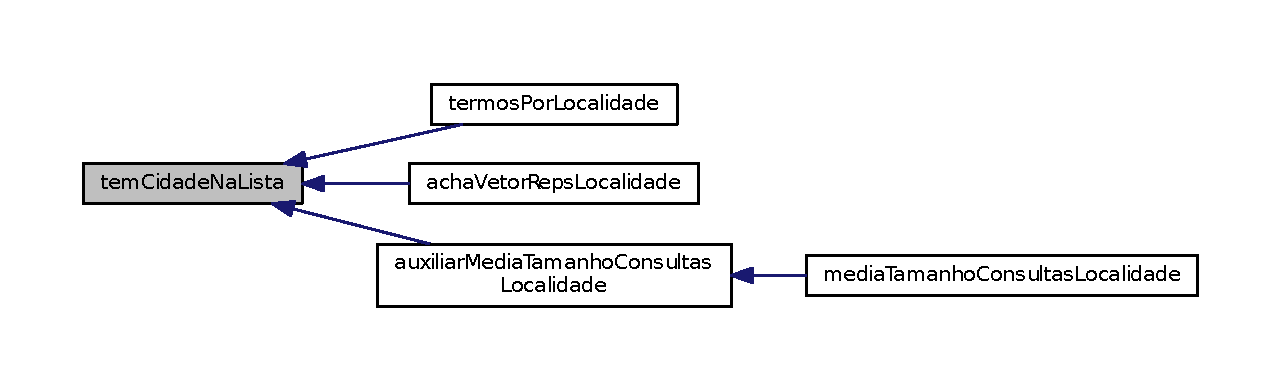
\includegraphics[width=350pt]{operacoes_8h_a3af226df14ca18acf9c3de7d605004d5_icgraph}
\end{center}
\end{figure}
\mbox{\Hypertarget{operacoes_8h_ac04e2f9df7f7b0f31c80a7aa7f76297d}\label{operacoes_8h_ac04e2f9df7f7b0f31c80a7aa7f76297d}} 
\index{operacoes.\+h@{operacoes.\+h}!termos\+Arquivo@{termos\+Arquivo}}
\index{termos\+Arquivo@{termos\+Arquivo}!operacoes.\+h@{operacoes.\+h}}
\subsubsection{\texorpdfstring{termos\+Arquivo()}{termosArquivo()}}
{\footnotesize\ttfamily \hyperlink{struct_8h_ae030205799002e4fc414e374283d8598}{L\+DE}$\ast$ termos\+Arquivo (\begin{DoxyParamCaption}\item[{\hyperlink{struct_8h_ae030205799002e4fc414e374283d8598}{L\+DE} $\ast$}]{lista\+Termos }\end{DoxyParamCaption})}



Encontra os termos consultados em um arquivo. 

A função \hyperlink{operacoes_8h_ac04e2f9df7f7b0f31c80a7aa7f76297d}{termos\+Arquivo()} encontra todos os termos que foram consultados em um arquivo.


\begin{DoxyParams}{Parâmetros}
{\em lista\+Termos} & Lista de todos os termos consultados no arquivo \\
\hline
{\em cidade} & Cidade a qual estamos procurando os termos\\
\hline
\end{DoxyParams}
\begin{DoxyReturn}{Retorna}
{\ttfamily L\+D\+E$\ast$} que é a lista de todos os termos consultados no arquivo. 
\end{DoxyReturn}
\begin{DoxyWarning}{Aviso}
Essa função é apenas um placeholder, para manter uma convenção de sempre chamarmos uma função para as operações, já que já temos todos os termos do arquivo separados em uma estrutura própria. 
\end{DoxyWarning}
\mbox{\Hypertarget{operacoes_8h_a8375d33a9e2f1d5a7fa40eadbfd59ad3}\label{operacoes_8h_a8375d33a9e2f1d5a7fa40eadbfd59ad3}} 
\index{operacoes.\+h@{operacoes.\+h}!termos\+Por\+Localidade@{termos\+Por\+Localidade}}
\index{termos\+Por\+Localidade@{termos\+Por\+Localidade}!operacoes.\+h@{operacoes.\+h}}
\subsubsection{\texorpdfstring{termos\+Por\+Localidade()}{termosPorLocalidade()}}
{\footnotesize\ttfamily \hyperlink{struct_8h_ae030205799002e4fc414e374283d8598}{L\+DE}$\ast$ termos\+Por\+Localidade (\begin{DoxyParamCaption}\item[{\hyperlink{struct_8h_a1664119ce88635d3bf4655a988ef8248}{Consulta} $\ast$}]{arvore,  }\item[{\hyperlink{struct_8h_ae030205799002e4fc414e374283d8598}{L\+DE} $\ast$}]{lista,  }\item[{char}]{cidade\mbox{[}$\,$\mbox{]} }\end{DoxyParamCaption})}



Encontra os termos consultados em uma localidade. 

A função \hyperlink{operacoes_8h_a8375d33a9e2f1d5a7fa40eadbfd59ad3}{termos\+Por\+Localidade()} encontra todos os termos que foram consultados em uma localidade. Funciona R\+E\+C\+U\+R\+S\+I\+V\+A\+M\+E\+N\+TE.


\begin{DoxyParams}{Parâmetros}
{\em arvore} & Arvore que contem os dados \\
\hline
{\em lista} & {\ttfamily L\+DE} onde serão inseridos os termos do nodo atual da arvore. \\
\hline
{\em cidade} & Cidade a qual estamos procurando os termos\\
\hline
\end{DoxyParams}
\begin{DoxyReturn}{Retorna}
{\ttfamily L\+D\+E$\ast$} que é a lista com todos os termos pesquisados naquela cidade. 
\end{DoxyReturn}
\begin{DoxyWarning}{Aviso}
Na primeira chamada dessa função, a {\ttfamily lista} precisa ser V\+A\+Z\+IA. 
\end{DoxyWarning}
Grafo de chamadas desta função\+:\nopagebreak
\begin{figure}[H]
\begin{center}
\leavevmode
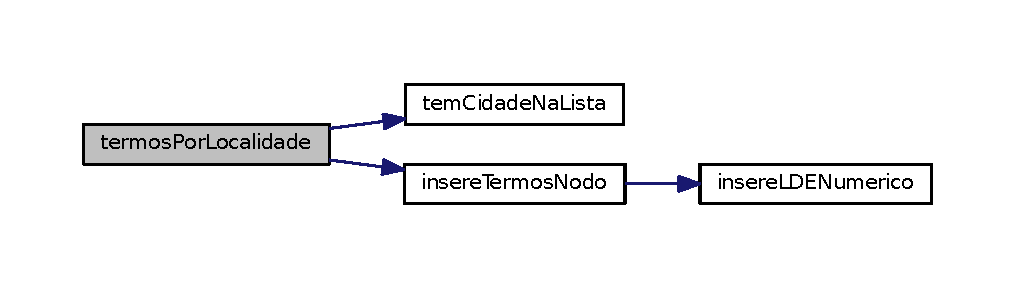
\includegraphics[width=350pt]{operacoes_8h_a8375d33a9e2f1d5a7fa40eadbfd59ad3_cgraph}
\end{center}
\end{figure}

\hypertarget{struct_8h}{}\section{Referência ao ficheiro struct.\+h}
\label{struct_8h}\index{struct.\+h@{struct.\+h}}


Arquivo que contém as estruturas utilizadas no programa.  


Este grafo mostra quais são os ficheiros que incluem directamente ou indirectamente este ficheiro\+:\nopagebreak
\begin{figure}[H]
\begin{center}
\leavevmode
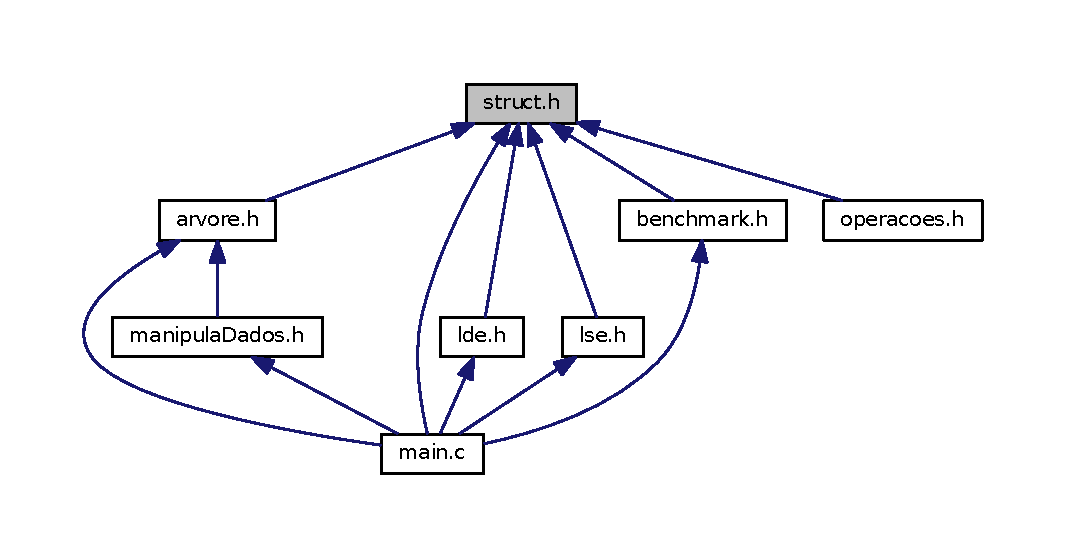
\includegraphics[width=350pt]{struct_8h__dep__incl}
\end{center}
\end{figure}
\subsection*{Estruturas de Dados}
\begin{DoxyCompactItemize}
\item 
struct \hyperlink{structlde}{lde}
\begin{DoxyCompactList}\small\item\em Lista duplamente encadeada. \end{DoxyCompactList}\item 
struct \hyperlink{structlse}{lse}
\begin{DoxyCompactList}\small\item\em Lista simplesmente encadeada. \end{DoxyCompactList}\item 
struct \hyperlink{structabp}{abp}
\begin{DoxyCompactList}\small\item\em Arvore binária. \end{DoxyCompactList}\item 
struct \hyperlink{structdescritor}{descritor}
\begin{DoxyCompactList}\small\item\em Estrutura principal do programa, responsável por guardar T\+O\+D\+OS os dados. \end{DoxyCompactList}\item 
struct \hyperlink{structs__qtd_cons}{s\+\_\+qtd\+Cons}
\begin{DoxyCompactList}\small\item\em Estrutura utilizada para guardar uma L\+SE e um valor numérico arbitrário. \end{DoxyCompactList}\end{DoxyCompactItemize}
\subsection*{Definições de tipos}
\begin{DoxyCompactItemize}
\item 
typedef struct \hyperlink{structlde}{lde} \hyperlink{struct_8h_ae030205799002e4fc414e374283d8598}{L\+DE}
\begin{DoxyCompactList}\small\item\em Lista duplamente encadeada. \end{DoxyCompactList}\item 
\mbox{\Hypertarget{struct_8h_a0d3de75d86bf1db6f749c91f755b870c}\label{struct_8h_a0d3de75d86bf1db6f749c91f755b870c}} 
typedef struct \hyperlink{structlse}{lse} \hyperlink{struct_8h_a0d3de75d86bf1db6f749c91f755b870c}{L\+SE}
\begin{DoxyCompactList}\small\item\em Lista simplesmente encadeada. \end{DoxyCompactList}\item 
typedef struct \hyperlink{structabp}{abp} \hyperlink{struct_8h_a1664119ce88635d3bf4655a988ef8248}{Consulta}
\begin{DoxyCompactList}\small\item\em Arvore binária. \end{DoxyCompactList}\item 
typedef struct \hyperlink{structdescritor}{descritor} \hyperlink{struct_8h_a1f5d65da7c19674431ada6dcf434b9ec}{Info}
\begin{DoxyCompactList}\small\item\em Estrutura principal do programa, responsável por guardar T\+O\+D\+OS os dados. \end{DoxyCompactList}\item 
typedef struct \hyperlink{structs__qtd_cons}{s\+\_\+qtd\+Cons} \hyperlink{struct_8h_a30e93d002c23d05f5d039449d6775eb6}{Qtdcons}
\begin{DoxyCompactList}\small\item\em Estrutura utilizada para guardar uma L\+SE e um valor numérico arbitrário. \end{DoxyCompactList}\end{DoxyCompactItemize}


\subsection{Descrição detalhada}
Arquivo que contém as estruturas utilizadas no programa. 

\mbox{\Hypertarget{struct_8h_a1664119ce88635d3bf4655a988ef8248}\label{struct_8h_a1664119ce88635d3bf4655a988ef8248}} 
\index{struct.\+h@{struct.\+h}!Consulta@{Consulta}}
\index{Consulta@{Consulta}!struct.\+h@{struct.\+h}}
\subsubsection{\texorpdfstring{Consulta}{Consulta}}
{\footnotesize\ttfamily typedef struct \hyperlink{structabp}{abp}  \hyperlink{struct_8h_a1664119ce88635d3bf4655a988ef8248}{Consulta}}



Arvore binária. 

Arvore binária de pesquisa responsável por guardar todos os dados das consultas. Cada nodo da árvore representa uma consulta, armazenando os termos da consulta, além das cidades que realizaram essa consulta.

\begin{DoxyWarning}{Aviso}
A árvore é binária de pesquisa, P\+O\+RÉM a chave dela não é tão útil para a realização das pesquisas. 
\end{DoxyWarning}
\mbox{\Hypertarget{struct_8h_a1f5d65da7c19674431ada6dcf434b9ec}\label{struct_8h_a1f5d65da7c19674431ada6dcf434b9ec}} 
\index{struct.\+h@{struct.\+h}!Info@{Info}}
\index{Info@{Info}!struct.\+h@{struct.\+h}}
\subsubsection{\texorpdfstring{Info}{Info}}
{\footnotesize\ttfamily typedef struct \hyperlink{structdescritor}{descritor}  \hyperlink{struct_8h_a1f5d65da7c19674431ada6dcf434b9ec}{Info}}



Estrutura principal do programa, responsável por guardar T\+O\+D\+OS os dados. 

Estrutura principal do programa, que guarda tanto a árvore binária de pesquisa {\ttfamily arvore}, como a lista geral de termos consultados {\ttfamily termos}. \mbox{\Hypertarget{struct_8h_ae030205799002e4fc414e374283d8598}\label{struct_8h_ae030205799002e4fc414e374283d8598}} 
\index{struct.\+h@{struct.\+h}!L\+DE@{L\+DE}}
\index{L\+DE@{L\+DE}!struct.\+h@{struct.\+h}}
\subsubsection{\texorpdfstring{L\+DE}{LDE}}
{\footnotesize\ttfamily typedef struct \hyperlink{structlde}{lde}  \hyperlink{struct_8h_ae030205799002e4fc414e374283d8598}{L\+DE}}



Lista duplamente encadeada. 

Lista duplamente encadeada, que pode ou não ser circular. \mbox{\Hypertarget{struct_8h_a30e93d002c23d05f5d039449d6775eb6}\label{struct_8h_a30e93d002c23d05f5d039449d6775eb6}} 
\index{struct.\+h@{struct.\+h}!Qtdcons@{Qtdcons}}
\index{Qtdcons@{Qtdcons}!struct.\+h@{struct.\+h}}
\subsubsection{\texorpdfstring{Qtdcons}{Qtdcons}}
{\footnotesize\ttfamily typedef struct \hyperlink{structs__qtd_cons}{s\+\_\+qtd\+Cons}  \hyperlink{struct_8h_a30e93d002c23d05f5d039449d6775eb6}{Qtdcons}}



Estrutura utilizada para guardar uma L\+SE e um valor numérico arbitrário. 

Estrutura que é utilizada somente na função \hyperlink{operacoes_8h_a51685935591ec37d31c3a5600fe3f721}{consultas\+Por\+Localidade()} para poder armazenar quantas vezes uma {\ttfamily L\+S\+E$\ast$} foi chamada. 
%--- End generated contents ---
% Index

\end{document}
